\chapter{Statistisk inferens: Forventninger og gjennomsnitt}
\label{kap:forventninger_og_gjennomsnitt} % Opprinnelig kapittelnr: 8

\section{Målemodellen}

En problemstilling som dukker opp i mange sammenhenger er:
En ukjent størrelse $\mu$ skal måles, men vi har erfart at gjentatte
målinger av $\mu$ vanligvis ikke gir samme resultat, selv om
vi forsøker å måle under de samme
forsøksbetingelser hver gang. Dette skyldes ofte en
ufullkommen metode, enten ved at måleverktøyet bare
måler med en begrenset nøyaktighet, eller andre
forstyrrende faktorer som ligger utenfor vår kontroll. I noen
situasjoner kan nøyaktig måling av $\mu$ være praktisk
(endog teoretisk) umulig. Vi sier at målingene er foretatt
med {\em målefeil}. Ved å foreta gjentatte målinger
håper vi at vi kan redusere den usikkerhet som er forbundet
med en enkelt måling. De første statistiske teorier på 
1700-tallet \footnote{Nøkkelpersonene var
matematikerne Laplace (1749-1827) og Gauss (1777-1855).}
tok nettopp sikte på å legge et teoretisk grunnlag for
behandling av målefeil.

Vi skal i dette avsnittet studere en enkel statistisk modell
som har vist seg fruktbar ved analyse av usikkerhet i målefeil.
Selv om modellen er gitt navnet {\em målemodellen},
har den langt bredere anvendelse og er i dag en del av grunnlaget for
usikkerhetsvurderinger ved observasjoner innen de fleste fagområder.

Siden vi skal ha en modell for måling under usikkerhet, er
det rimelig å formulere en stokastisk modell: En måling
av en ukjent størrelse $\mu$ oppfattes som en realisasjon av
en stokastisk variabel $X$ med forventning $\mu$. Foretar vi
$n$ gjentatte målinger av $\mu$, kan vi oppfatte disse som
realisasjoner av $n$ stokastiske variable $X_1, X_2,\ldots ,X_n$
alle med samme forventning $\mu$. Det er ofte rimelig å anta at
usikkerheten i hver måling er den samme. Vi uttrykker dette i modellen
ved å anta at de stokastiske variable  $X_1, X_2,\ldots ,X_n$
har den samme varians, kall den $\sigma ^2.$ Videre er det ofte
rimelig å anta at målingene ikke avhenger av hverandre.
Vi uttrykker dette i modellen ved å anta at
$X_1,X_2,\ldots ,X_n$ er uavhengige stokastiske variable (se
Kapittel 5.6). Vi har derfor:
\begin{center} \framebox[10cm]{\begin{minipage}{9cm}\rule{0cm}{0.5cm}
     {\bf Målemodellen:} $X_1,X_2,\ldots ,X_n$ er $n$
     uavhengige stokastiske variable der
     \[  EX_1=EX_2=\cdots =EX_n=\mu       \]
     \[  varX_1=varX_2=\cdots =varX_n=\sigma^2.\]
\mbox{}
\end{minipage}} \end{center}
I denne modellen er $\mu$ og $\sigma ^2$ parametre hvis verdier
vanligvis er ukjente. Hensikten med å foreta de $n$
målingene er nettopp å få informasjon om $\mu$ og
helst også om $\sigma ^2$, dersom denne også er ukjent.
Eksempler på situasjoner hvor målemodellen kan være
realistisk er:
\begin{itemize}
\item   Gjentatte veiinger av en gjenstand med sann vekt
     $\mu$. $\sigma^ 2$ uttrykker da usikkerheten i hver veiing.
\item   Alkoholkonsentrasjonen i $n$ blodprøver tatt på samme
     person. $\mu$ er den ``sanne promille", og $\sigma ^2$
     uttrykker usikkerheten i en enkelt blodprøve.
\item   Måling av strekkstyrken av $n$ nylonsnører av en
     bestemt type.  Her er $\mu$ gjennomsnittlig strekkstyrke av
     slike nylonsnører, mens $\sigma ^2$ uttrykker variasjonen
     i strekkstyrke fra snøre til snøre.
\item   Bestemmelse av kvikksølvkonsentrasjonen i $n$ lagesild
     oppfisket fra Mjøsa. Her uttrykker $\mu$ den
     gjennomsnittlige konsentrasjon av kvikk\-sølv hos lagesild
     i Mjøsa, mens $\sigma^ 2$ uttrykker variasjonen i
     konsentrasjonen.
\end{itemize}
Merk at de to første eksemplene dreier seg om usikkerhet i
form av målefeil, mens det tredje eksemplet dreier seg om
usikkerhet ved at de målte objekter kun er representanter fra
en større, prinsipielt uendelig, populasjon med en viss
innbyrdes variasjon. Det samme gjelder det siste eksemplet. I de
to siste eksemplene vil variansen $\sigma ^2$ også kunne
inneholde en viss komponent av direkte målefeil, men denne
vil vanligvis være neglisjerbar i forhold til de individuelle
variasjoner hos måleobjektene.
\footnote{Eksempel 6 i Kapittel 1 vil
også kunne motivere deg for teorien i dette avsnittet, og
anbefales lest (evt. repetert) nå.}

I alle eksemplene kan den aktuelle variable måles på en
prinsipielt kontinuerlig skala, selv om resultatet i praksis 
måles på en diskret skala, f.eks. kvalitet (strekkstyrke)
av et produkt målt i kilo med to desimaler. Målemodellen
tillater imidlertid diskrete variable, f.eks antall registrerte feil
ved et produkt.

I praksis ser man ofte data på en vurderingsskala, f.eks kvalitet
vurdert i kategorier fra 1 til 7. Da er det ikke lenger sikkert at
analyse basert på målemodellen er meningsfull. Kan hende
reflekterer tallene bare såkalte {\em ordinale} egenskaper ved
kvaliteten, at 2 er bedre enn 1 osv. Det har da liten mening å
bruke begrepet forventet kvalitet. Det kan imidlertid være 
grensetilfeller der det kan diskuteres om ikke målemodellen
likevel kan brukes. Betrakt følgende to situasjoner:\\
\indent 1. En kontrollør vurderer $n$ produkter i den 
løpende produksjon.\\
\indent 2. Et produkt eller en tjeneste blir vurdert av n kunder.\\
I den første situasjonen kan en nok tenke seg at retningslinjer for
skale\-ring er gitt, slik at målemodellen kan brukes. Den andre
situasjonen er mer problematisk, spesielt fordi ulike kunder ikke
nødvendigvis legger det samme i kategoribeskrivelsene, f.eks.
1=helt ubrukelig, 2=nesten ubrukelig osv.
Det fins en omfattende litteratur om vurderingsskalaer
(hovedsakelig med utgangspunkt i psykologi) som søker å
løse dette problem, enten ved å etablere skaleringsmetoder
slik at målemodellen likevel kan brukes, eller ved å
basere analysen på alternative modeller.
  
La oss i første omgang studere problemet å estimere $\mu$
på basis av de $n$ observasjonene $X_1,X_2,\ldots X_n$. I
praksis har det ofte vært vanlig å bruke gjennomsnittet
av observasjonene

\[  \hat{\mu}=\bar{X}=\frac{1}{n}(X_1+X_2+\cdots +X_n) \]
som estimator for den felles forventning $\mu$.  Denne estimatoren har bl.a.
følgende egenskaper
\begin{center} \framebox[10cm]{\begin{minipage}{9cm}
\[  E(\bar{X})=\mu \mbox{\ \ \ \ \ \ \ \ } var(\bar{X})=\frac{\sigma ^2}{n} \]
\mbox{}
\end{minipage}} \end{center}
Vi ser at $\bar X$ er en forventningsrett estimator for $\mu$, med varians
som avhenger av variansen til enkeltobservasjonene og antall observasjoner.\\

\noindent {\bf Begrunnelse:}
Merk de overganger der vi benytter modellantakelser
\small
\begin{eqnarray*}
   E(\bar{X})&=&E({1\over n}(X_1+X_2+\cdots +X_n))=
              {1\over n}E(X_1+X_2+\cdots+ X_n)\\
             &=&{1\over n}(EX_1+EX_2+\cdots +EX_n)=
              {1\over n}(\mu+\mu+\cdots+ \mu)\\
             &=&{1\over n}\cdot n\cdot \mu=\mu.\\
 var(\bar X)&=&var({1\over n}(X_1+X_2+\cdots +X_n))
            =\left({1\over n}\right)^2var (X_1+X_2+\cdots +X_n)\\
            &=&\left({1\over n}\right)^2(varX_1+varX_2+\cdots +varX_n)\\
      &=&({1\over n})^2(\sigma ^2+\sigma ^2+\cdots +\sigma ^2)
            =({1\over n})^2n\sigma ^2 ={\sigma ^2\over n}.
\end{eqnarray*}
\normalsize
Ved vurdering av påliteligheten til $\bar X$ som estimator for $\mu$
bruker vi standardavviket til $\bar X$. Vi har
\begin{center} \framebox[10cm]{\begin{minipage}{9cm}\rule{0cm}{0.5cm}
{\bf Kvadratrotloven :  } 
\[  \Delta =\sigma (\bar X)={\sigma \over \sqrt n}. \]
\mbox{}  \end{minipage}} \end{center}
Estimatoren kan gjøres så presis man ønsker ved å
ta et tilstrekkelig stort antall observasjoner.
Imidlertid sier kvadratrotloven at vi, for å halvere usikkerheten
 målt ved standardavviket, må firedoble antall observasjoner.

Siden $\bar{X}$ oppfyller betingelsene i sentralgrensesetningen, 
kan vi bruke normaltilnærming såframt $n$
ikke er for liten (se Kapittel 6.5). Vi får 

\[ P(\mid \bar X - \mu \mid < k\cdot \sigma (\bar X))\approx A(k)  \]
På samme måte som i forrige kapittel, kan dette brukes til
å lage sannsynlighetsutsagn om estimeringsfeilen. Også
her er det rimelig å rapportere

\[   \mbox{estimat $\pm$ standardavviket til estimatoren}   \]
som i denne situasjonen blir

\[ \bar X \pm \sigma (\bar X) \mbox{\ \ \ \ der \ \ \ } 
                       \sigma (\bar X)={\sigma \over \sqrt n}\]

\begin{eksempel}{Alkotest}
En bestemt metode til å måle alkoholkonsentrasjon i blod
er forbundet med en betydelig usikkerhet. Følgelig tas det
gjentatte målinger. Anta at en enkelt måling kan
oppfattes som realisasjon av en stokastisk variabel $X$ med
forventning den ``sanne" alkoholkonsentrasjon  $\mu$ i promille
og med standardavvik lik $\sigma$. Fra tidligere erfaring har det
vist seg at $\sigma=0.20$ uansett hvilken $\mu$ vi har. La oss
anta at vi har tatt $n=3$ målinger hos en person rett etter
hverandre, og betegn disse med $X_1,X_2,X_3$. Vi ønsker på
dette grunnlag å estimere $\mu$. Dersom det er rimelig å
anta at observasjonene er uavhengige av hverandre, har vi et
tilfelle av målemodellen. Anta at observasjonene var
\begin{center}
\begin{tabular}{ccc}
    0.40 &  0.65 & 0.75
\end{tabular}
\end{center}
Her blir $\bar X = {1\over 3}(0.40 + 0.65 + 0.75)=0.60$ og
$\sigma(\bar X)=0.20/{\sqrt 3}=0.115$, og vi rapporterer derfor at
alkoholkonsentrasjonen er

\[     0.60 \; \; \pm \; \; 0.115 \]
Jeg tror ikke jeg ville ta sjansen på å sikte vedkommede
på dette grunnlag (i hvertfall ikke dersom forsvareren har
litt greie på statistikk).
\end{eksempel}

For å kunne angi standardavviket $\sigma (\bar X)$ til
estimatoren må vi kjenne standardavviket $\sigma$ til
enkeltmålingene. I mange situasjoner er imidlertid $\sigma$
helt eller delvis ukjent. Vi må da nøye oss med et anslag
for $\sigma$. Noen ganger kan man utnytte informasjon fra
tidligere, om tilsvarende målinger foretatt med om lag samme
presisjon. Uten slik informasjon er vi henvist til å
anslå $\sigma$ på grunnlag av de foreliggende
observasjonene. La oss forsøke å finne en brukbar
estimator for $\sigma ^2$ på grunnlag av observasjonene 
$X_1,X_2,\ldots, X_n$. Vi har

\[\sigma ^2=E{(X_1-\mu )}^2=E{(X_2-\mu )}^2=\cdots =E{(X_n-\mu )}^2\]
Herav følger at $E({1\over n}\sum_{i=1}^n(X_i-\mu )^2)=\sigma ^2$.
Hadde $\mu$ vært kjent ville derfor

\[  {1\over n}\sum_{i=1}^n{(X_i-\mu )}^2 \]
være en forventningsrett estimator for $\sigma ^2$. Når
$\mu$ er ukjent erstatter vi $\mu$ med sin estimator $\bar X$
i dette uttrykket, og håper på at

\[ S_X^2={1\over n}\sum_{i=1}^n{(X_i-\bar X)}^2      \]
er en brukbar estimator for $\sigma ^2$. Denne
størrelsen kalles ofte for {\em den empiriske varians.} Vi ser
at den empiriske varians gir uttrykk for spredningen av de $n$
observasjonene. Den er det empiriske motstykke til det
modell\-teoretiske begrep varians.\
\footnote{I situasjoner der det ikke er behov for å skille mellom 
(teoretisk) varians og empirisk varians sløyfes gjerne ordet empirisk
 (Jfr. Kapittel 1.3.)}
 Kvadratroten av $S_X^2$, kalt $S_X$, omtales ofte
som {\em det empiriske standardavvik}. Den empiriske varians kan
også uttrykkes på andre måter, som i en gitt
situasjon kan være mer velegnet for bereg\-nings\-formål (se
f.eks. Oppgave~\ref*{kap:introduksjon}.11). 

Vi vil studere den foreslåtte estimator
litt nærmere, og spør først om $S_X^2$ er en
forventningsrett estimator for $\sigma ^2$. Det viser seg at (se
 $\star$-merket stoff til slutt i avsnittet)

\[  E(S_X^2)={n-1\over n}\sigma ^2   \]
slik at den foreslåtte estimator ikke er forventningsrett.
Faktoren $(n-1)/n$ nærmer seg $1$ når $n$ vokser, og
skjevheten gjør seg derfor bare gjeldende for små $n$. Vi
sier at estimatoren er asymptotisk forventningsrett. Det funne
resultat viser imidlertid at skjevheten kan korrigeres ved å
dividere med $n-1$ istedenfor $n$.
Det er vanlig å bruke den korrigerte kvadratsummen som
estimator for $\sigma ^2$ med betegnelsen $S^2$, og å
omtale denne som den empiriske varians. Noen legger mindre vekt
på forventningsretthet, og lar være å foreta korreksjon.
Vi ser at ulik praksis bare slår ut for små $n$.

Anta at vi har valgt å bruke $\bar X$ som estimator for
$\mu$, og at $\sigma$ på forhånd er ukjent, slik at vi
må bruke våre observasjoner også til å estimere
$\sigma$. Anta at vi har valgt den forventningsrette 
     
\[   S^2={1\over {n-1}}\sum_{i=1}^n(X_i-\bar X)^2\]
som estimator for $\sigma ^2$. Det er da vanlig å bruke
 $S=\sqrt{S^2}$ som estimator for $\sigma$, og videre bruke

     \[S(\bar X)={S\over \sqrt n}\]
som estimator for standardavviket $\sigma(\bar X)=\sigma/ \sqrt n$
til $\bar X$. Resultatet av estimeringen kan vi da rapportere slik

\[   \bar X \;\;\; \pm \;\;\; S(\bar X)   \]
Sannsynligheten for en estimeringsfeil mindre enn $k$ ganger
estimert standardavvik blir

\[    P(\mid \bar X -\mu \mid < k\cdot S(\bar X)) \]
Siden det ligger en viss risiko i å erstatte $\sigma$ med S,
må vi vente at denne sannsynligheten, for gitt $k$, blir noe
mindre enn den vi hadde når $\sigma$ var kjent, nemlig $A(k)$.
Imidlertid vil vi, dersom $n$ ikke er for liten, kunne vente at S
ligger nær $\sigma$, slik at tilnærmelsen $A(k)$ fortsatt
kan gi en pekepinn om faren for estimeringsfeil. For ytterligere
kommentarer, se Kapittel 8.5.\\

\begin{eksempel}{Strekkstyrke}
Vi ønsker å undersøke en bestemt type nylonsnøre mht.
strekkstyrken, og har innkjøpt $10$ snører av
denne typen. La $X_1,X_2,\ldots ,X_{10}$ være strekk\-styrken i kg
for de $10$ snørene. Anta at målemodellen er realistisk,
og at $\mu =EX_i$ gir uttrykk for gjennomsnittlig strekkstyrke for
snører av denne typen, mens $\sigma ^2=varX_i$ gir uttrykk for
tilfeldig variasjon fra snøre til snøre. Forutsetningen om
uavhengighet kan være tvilsom dersom snørene er valgt ut
på en spesiell måte, f.eks. dersom de er produsert rett
etter hverandre. Snører av dårlig kvalitet kan da komme
samlet, f.eks. ved at maskinene er dårlig justert, eller at
råstoffet tilfeldigvis var av dårligere kvalitet enn vanlig.
Anta at observasjonene er gitt ved
\begin{center}
\begin{tabular}{cccccccccc}
   9.36&9.75&9.23&10.32&10.07&9.68&9.96&9.70&10.15&9.68
\end{tabular}
\end{center}
Vi får $\bar X=9.79$ og $S=0.34$, slik at $S(\bar X)=S/\sqrt{10}=0.11$.
Vi rapporterer at gjennomsnittlig strekkstyrke er
$9.79\pm 0.11$.
\end{eksempel}

Et interessant spørsmål i forbindelse med dette eksemplet
vil være: Anta at vi plukker ut et nytt snøre og belaster
det med 10 kg. Hva er sannsynligheten for at det ryker. La $X$
være strekkstyrken til dette snøret. Vi skal altså finne
$P(X < 10.0)$. En beregning basert på estimert forventning  9.79
og estimert standardavvik 0.34 og normaltilnærmelse, vil gi en
sannsynlighet på 0.73. De estimerte verdier er åpenbart
nokså usikre, og bør helst ikke brukes i ``eksakte" 
sannsynlighetsberegninger av denne typen, med mindre de er basert på 
et langt større erfaringsmateriale (se likevel Kapittel 16.5).

Vi har sett at presisjonen av estimatet vil øke med antall
observasjoner. Dersom vi ønsker en viss presisjon må vi
sørge for å ta tilstrekkelig mange observasjoner. På
den annen side vil for mange observasjoner være sløsing
med ressurser (tid, evt. penger). Ønsker vi at estimatoren
skal ha stan\-dard\-avvik $\Delta$, er antall observasjoner gitt ved
formelen

\[   n=\frac{\sigma ^2}{\Delta ^2}. \]
For å bruke formelen trenger vi å kjenne $\sigma$, dvs.
usikkerheten i hver enkelt observasjon. Noen ganger er denne
kjent fra tidligere observasjoner foretatt med om lag samme
usikkerhet. Uten slik informasjon kan man foreta en
forundersøkelse basert på et mindre antall observasjoner.
Vi vil som regel være fornøyd med å bestemme
størrelsesorden av $n$, og et grovt anslag for $\sigma$ vil
derfor være tilstrekkelig. Under alle omstendigheter vil litt
forsøksplanlegging være bedre enn ingen
forsøkplanlegging.

La oss så gå over til å studere testing av hypoteser
om forventninger i målemodeller.\\

\begin{eksempel}{Testing av forbedring}
Anta vi etter omfattende målinger har anslått at den
gjennomsnittlige kvikksølvkonsentrasjon hos en fiskeart i en
innsjø er $17.2$ enheter. Etter dette er det iverksatt
restriksjoner på utslippet av avfall, og etter en tid ønsker vi å
undersøke om det er noen påviselig reduksjon i
kvikksølvkonsen\-trasjon. Variasjonen i konsentrasjon fiskene i mellom
har hittil svart til et stan\-dard\-avvik $\sigma$ omtrent lik $1.5$. 
Feilen ved måling av den enkelte fisk er neglisjerbar i forhold til dette.
Det er bestemt å undersøke $n=9$ fisk.
Problemet kan formuleres som et testproblem i en målemodell.
\end{eksempel}

I generelle termer studerer vi følgende problem for
målemodellen:
La $X_1, X_2,\ldots ,X_n$ være $n$ uavhengige observasjoner fra
samme sannsynlighetsfordeling hvor forventningen $\mu$ er ukjent,
mens variansen $\sigma ^2$ antas kjent. Vi ønsker å teste
om $\mu$ er lik en gitt verdi $\mu_0$ mot alternativet at $\mu$
er mindre enn verdien ${\mu}_0$, dvs.

\[ H_0:\mu ={\mu}_0 \mbox{\ \ mot \ \ } H_A:\mu < {\mu}_0.\]
Ved valg av testmetode vil vi ta utgangspunkt i 

\[  \bar X={1\over n}\sum_{i=1}^n X_i\]
som vi vet er en brukbar estimator for $\mu$. En rimelig
testmetode vil være å forkaste $H_0$ og påstå
$H_A$ når $\bar X$ er liten i forhold til ${\mu}_0$, hvor liten
vil avhenge av hvilke risker for feilkonklusjon vi er villig til
å løpe. Som testobservator er det hensiktsmessig å
bruke 

\[Z =\frac{\bar{X}-{\mu}_0}{ \sigma (\bar{X})}=\frac{\bar X -{\mu}_0}
                                    {\sigma /\sqrt{n}}     \]
og testmetoden lar vi være:

\[ \mbox{Forkast $H_0$ og påstå $H_A$ dersom $Z\le k$} \]
der $k$ er en passende valgt konstant. Anta at vi ønsker
signifikansnivå $\alpha$. Vi må da velge $k$ slik at 

\[  P_{H_0}(Z\le k)=\alpha        \]
For bestemmelse av $k$ må vi derfor kjenne
sannsynlighetsfordelingen til $Z$ under forutsetning av at $H_0$
er riktig. Eksakt bestemmelse er ikke mulig uten ekstra
forutsetninger om de stokastiske variable i modellen (mer om
dette i Kapittel 8.4). Her må vi nøye oss med
tilnærmet beregning: Anta at $n$ er så stor at vi kan
forsvare å bruke normaltilnærming (se Kapittel 6.5).
Under forutsetning av at $H_0$ er riktig vil histogrammet til $Z$
kunne tilnærmes med normalkurven (fordi da er $Z$ den
korrekte standardisering av $\bar X)$. Vi får derfor 

\[      P_{H_0}(Z\le k)\approx G(k)\]
Ved å bestemme $k$ av ligningen $G(k)=\alpha$, får vi
derfor en test med tilnærmet signifikansnivå $\alpha$, se Figur~\ref{fig:kritisk_verdi}.
Eksempelvis dersom vi krever $\alpha=0.05$, blir $k={-1.645}$,
mens dersom vi krever $\alpha =0.01$, blir $k=-2.326$.

\begin{figure}[ht]
\centering
	\includegraphics[scale=1.0]{figurer/fig8_1.pdf} 
 \caption{Bestemmelse av kritisk verdi}
	\label{fig:kritisk_verdi}
\end{figure}
\noindent Merk at testmetoden kan alternativt skrives som 
\[  \mbox{Forkast $H_0$ og påstå $H_A$ dersom $\bar X\le 
                          {\mu}_0 - k_{\alpha} \cdot \sigma /\sqrt n$} \]
der $k_{\alpha}$ det  positive tall som har areal $\alpha$ til høyre for seg
under normalkurven (her er $k=-k_{\alpha}$). Vi ser at hvor mye mindre $\bar X$ må være enn
${\mu}_0$ før vi våger å forkaste $H_0$,
vil avhenge av antall observasjoner $n$, usikkerheten i hver
enkelt observasjon $\sigma$ og signifikansnivået $\alpha$.

Vi vil også være interessert i styrken til testen,
dvs. evnen til å avsløre at $\mu < {\mu}_0$, dersom $\mu$ i
virkeligheten er slik. Styrkefunksjonen blir 

\begin{eqnarray*}
\Pi (\mu )&=&P(\mbox{forkaste $H_0$})=P(Z\le -k_{\alpha})\\
          &=&P(\bar X \le {\mu}_0 - k_{\alpha}\cdot \sigma /\sqrt {n})\\
          &=&P(\frac{\bar X - \mu}{\sigma /\sqrt{n}} \le
          \frac{{\mu}_0 - \mu}{\sigma /\sqrt{n}}-k_{\alpha})\\
  &\approx& G(\frac{{\mu}_0 - \mu}{\sigma /\sqrt{n}}-k_{\alpha})
\end{eqnarray*}
Vi har her brukt normaltilnærming på sannsynlighetsfordelingen til \\
$(\bar X - \mu)/(\sigma /\sqrt{ n})$,
som er den standardiserte variable til $\bar X$ uansett hva $\mu$ er.
Vi ser at $\Pi (\mu )$ er en avtagende funksjon av $\mu$
og at $\alpha =\Pi ({\mu}_0)$. Generelt vil styrken
avhenge av $\alpha$ (via $k_{\alpha}$) og av $\mu$, $\sigma$ og $n$ (via
størrelsen $({\mu}_0-\mu )/(\sigma \sqrt {n}))$.

\begin{figure}[ht]
\centering
  \includegraphics[scale=0.8]{figurer/fig8_2.pdf} 
 \caption{Styrkekurve}
	\label{fig:styrkekurve}
\end{figure}

\addtocounter{eksecount}{-1}
\begin{eksempel}{Testing av forbedring (fortsatt)}
I Eksempel 3 var ${\mu}_0=17.2$ og $\sigma =1.5$. Med $n=9$ og
$\alpha =0.05$ blir $k=-1.645$, som svarer til å forkaste
$H_0$ når $\bar X \le 16.38$. Styrkefunksjonen til denne
testen blir

\[ \Pi (\mu )\approx G(\frac{16.38-\mu}{0.5})   \]
La oss tabellere denne for noen $\mu$-verdier:
\begin{center} \addtolength{\tabcolsep}{-0.3\tabcolsep}
\begin{tabular}{c|cccccccc}
 $\mu$     & 14.5 & 15.0 & 15.5 & 16.0 & 16.5 & 17.0 & 17.2 & 17.5 \\ \hline
 $\Pi (\mu)$ &0.9999&0.9971&0.9604&0.7749&0.4032&0.1065&0.0500&0.0130
\end{tabular}
\end{center}
Styrkekurven er skissert i Figur~\ref{fig:styrkekurve}.

Eksempelvis ser vi at $\Pi (16.0)=0.7749$, dvs. at dersom $\mu$ er
redusert til $16.0$, er det en sannsynlighet på $1-
0.7749=0.2251$ for at vi ikke oppdager at det har foregått en
reduksjon i det hele tatt (godtakingsfeil). Vi merker oss forøvrig
at for $\mu>17.2$ blir $\Pi(\mu)< \alpha$, slik at
$\alpha$ blir en øvre skranke for forkastningsfeil også
når nullhypotesen er status quo eller forverring, og vi
ønsker å se om det er noen grunn til å påstå
forbedring, dvs. at situasjonen er å teste
$H_0:\mu \ge {\mu}_0 \mbox{\ \ mot \ \ } H_A:\mu < {\mu}_0.$
\end{eksempel}\\

I dette eksemplet var antall observasjoner $n$ gitt. En test som oppfyller 
både et gitt krav til forkastningsfeil $\alpha$ og godtakingsfeil $\beta$,
krever planlegging av $n$. En formel basert på  normaltilnærming er:
\[  n=(\frac{k_{\alpha} + k_{\beta}}{\mu_1 - \mu_0})^2 \cdot {\sigma}^2   \]
der $\mu_1$ er det valgte alternativ, der en ønsker en gitt $\beta$-risiko.
Her er $k_{\alpha}$ og $k_{\beta}$ punkter med de angitte arealer til høyre
for seg under normalkurven. For anvendelse av formelen se Oppgave~5. \\

\noindent Noen merknader om testing i målemodellen:
                                                   
1. I enkelte situasjoner er det aktuelt å teste
nullhypotesen $\mu={\mu}_0$ (eventuelt $\mu\le{\mu}_0)$ mot
alternativet $\mu> {\mu}_0$, se Oppgave~6. Da forkaster en nullhypotesen 
når $Z$ er større enn en kritisk verdi $k$, som i dette tilfellet bli 
$k=k_{\alpha}$. Formlen for planlegging av antall observasjoner er den samme.
Vi overlater til leseren å utarbeide detaljene, se Oppgave~9. 

2. I noen situasjoner kan det være aktuelt med såkalt to-sidig
test, dvs.\ at alternativet til nullhypotesen $\mu={\mu}_0$ er
$\mu\not={\mu}_0$, se Oppgave~8. Da forkaster en nullhypotesen når 
$\mid Z\mid$ er større enn en kritisk verdi $k$, dvs.\ både når $Z$ 
er liten og når $Z$ er stor. I dette tilfellet blir $k=k_{\alpha/2}$.
Samme planleggingsformel kan (tilnærmet) brukes for $n$, men erstatt
$\alpha$ med ${\alpha}/2$. Leseren kan selv utarbeide detaljene, se Oppgave~9.

3. Vi har i målemodellen hittil bare studert tester for
forventning $\mu$ for gitt varians $\sigma ^2$. Man kan også
formulere hypotesetestingsproblemer for variansen i
målemodellen. Et praktisk eksempel vil være en
produksjons\-prosess som, når den er i kontroll, gir artikler
av en gitt forventet kvalitet ${\mu}_0$, mens variansen $\sigma ^2$
er gitt lik ${\sigma}_0^2$. Kan hende løper prosessen ut av
kontroll ved at variansen har økt til et nivå større
enn ${\sigma}_0^2$, dvs. prosessen gir mer varierende kvalitet
enn før. Situasjonen kan studeres som et
hypotese\-testingsproblem om $\sigma ^2$ hvor nullhypotesen er
$\sigma ^2={\sigma}_0^2$ og alternativet er $\sigma ^2 > {\sigma}_0^2$.
Vi har ikke etablert nok teori til å behandle dette problem.

4. Vi har sett på testing av forventning i målemodellen
når variansen $\sigma ^2$ var kjent. I de fleste praktiske
situasjoner vil imidlertid $\sigma ^2$ være ukjent. Vi har
ikke etablert nok teori til å gjennomføre en grundig
diskusjon av denne problemstillingen, men siden den er så
viktig, vil vi gjengi de viktigste resultatene i Kapittel 8.4. 

5. Målemodellen kan legges til grunn for ulike betraktninger i forbindelse
med prosesstyring. I denne sammenheng er en både interessert i endringer i
forventning (nivå) og varians (spredning). Det praktiske verktøyet er
{\em kontrolldiagrammer}, der observasjonene plottes i naturlig rekkefølge,
og grenser for den naturlige variasjon tegnes inn, se Kapittel 15.
Regler for ``å gripe inn" ved avvikende mønstre kan da etableres
basert på sannsynlighetsbetraktninger, som gir visse garantier mot
feilaktig å gripe inn osv. \\[0.1cm]


 $\star$ \small  Estimatoren $\hat{\mu} = \bar X$ har en interessant egenskap:
Den er minste kvadraters estimatoren for forventningen $\mu$ i
målemodellen, som innebærer at den minimerer kvadratsummen
\[ Q(\mu )=\sum_{i=1}^n{(X_i-\mu)}^2 \]
Dette er en direkte følge av likheten (se Oppgave~27~(a))
\[  \sum_{i=1}^n{(X_i-\mu)}^2=
       \sum_{i=1}^n{(X_i-\bar X)}^2+n{(\bar X-\mu)}^2.\]
som viser at
\[  Q(\mu )\ge \sum_{i=1}^n{(X_i-\bar X)}^2.\]
med likhet hvis og bare hvis $\mu$ velges lik $\hat\mu=\bar X$.

Dette blir ofte sett på som en gunstig egenskap ved $\bar X$,
den føyer tallmaterialet på en bra måte, i den forstand
at den gjennomsnittlige kvad\-rerte avstand fra observasjonene til
estimatet for $\mu$ blir lite. Minimeringen av kvadratsummen
ovenfor er en anvendelse av et generelt prinsipp for utledning av
estimatorer kalt {\em minste kvadraters metode}, som spiller en
sentral rolle i statistisk teori. Imidlertid bør det advares
mot å legge for stor vekt på at en estimator er minste
kvadraters estimator. Det fins andre generelle prinsipper for
utledning av estimatorer, og en estimator bør alltid vurderes
i lys av den modell vi er villig til å anta. For ytterligere
kommentarer se Kapittel 8.4.

Formelen ovenfor kan også brukes ved beregning av
forventningen til den empiriske varians. Vi har

\[ S_X^2={1\over n}\sum_{i=1}^n {(X_i-\bar X)}^2= {1\over
               n}\sum_{i=1}^n {(X_i-\mu)}^2-{(\bar X-\mu)}^2.\]
Dette gir
\begin{eqnarray*}
  E(S_X^2)=E({1\over n}\sum_{i=1}^n {(X_i-\mu)}^2 )-
     E{(\bar {X}- \mu )}^2= \sigma ^2 - \sigma ^2/n=(n-1)/n \cdot
     \sigma ^2.
\end{eqnarray*}
\normalsize

\section{Lotterimodellen.}

I praksis støter en ofte på situasjoner hvor vi ønsker
å trekke slutninger om en gitt endelig populasjon på
grunnlag av et utvalg av elementer fra populasjonen. La oss nevne
noen eksempler:
\begin{itemize}
\item Vi kan finne ut noe om ungdommens røykevaner i en gitt
aldersgruppe i Bergen ved å spørre et utvalg av ungdommer.
\item Vi kan finne ut noe om årsinntekten til et kull
siviløkonomer $5$ år etter eksamen ved å ta for oss et
utvalg av slike.
\item Vi kan anslå volumet av trevirket i en skog ved å
måle et utvalg av trærne i skogen.
\end{itemize}

En slik framgangsmåte kalles ofte for en {\em
utvalgsundersøkelse}. Grunnen til at man foretar en
utvalgsundersøkelse framfor å innhente opplysninger om
alle elementene i populasjonen, kan være at det siste er
tidkrevende og/eller kostbart. Det finnes derfor en god del
teoretisk litteratur om ulike utvalgsmodeller og utvalgsmetoder.
Slike utvalgsmodeller danner et felles teoretisk grunnlag for en
rekke ulike anvendelser, eksempelvis intervjuundersøkelser,
meningsmålinger, markedsundersøkelser, kvalitetskontroll,
stikkprøverevisjon etc. Vi skal her se på en 
enkel (men nyttig) utvalgs\-modell som vi i det følgende vil
kalle {\em lotterimodellen}. Først litt notasjon:
   
Gitt en populasjon bestående av $N$ elementer. Til hvert element er
knyttet en verdi $v$. Vi tenker oss elementene nummerert fra $1$ til $N$,
og lar $v_i$ betegne $v$-verdien til element nr.$i$.
 Fra populasjonen trekkes et ordnet utvalg på $n$ elementer
(uten tilbakelegging). La $Y_j$ betegne $v$-verdien til det
j'te uttrukne element i utvalget $(j=1,2,\ldots ,n)$.

I de fleste anvendelser spiller rekkefølgen av elementene i
populasjon og utvalg ingen rolle, og nummereringen er bare av praktisk natur.

\begin{center} \framebox[10cm]{\begin{minipage}{9cm}\rule{0cm}{0.5cm}
{\bf Lotterimodellen:} Når verdiene $Y_1,Y_2,\ldots ,Y_n$ er bestemt 
som et {\em tilfeldig ordnet utvalg} fra $\{v_1,v_2,\ldots , v_N\}$.
sier vi at observasjonene oppfyller betingelsen i lotterimodellen. \\
\mbox{}
\end{minipage}} \end{center}                               
På grunnlag av $v$-verdien til de $n$ elementene utvalget
$Y_1,Y_2,\ldots ,Y_n$, ønsker vi å slutte noe om $v$-verdiene
til de $N$ elementene i populasjonen $v_1,v_2,\ldots ,v_N$.
Spesielt vil vi være interessert i å estimere den
gjennom\-snittlige $v$-verdi i populasjonen
     \[{\bar v}={1\over N}\sum_{i=1}^N v_i.\]
Som estimator er det rimelig å velge det tilsvarende
gjennomsnitt i  utvalget:

     \[{\bar Y}={1\over n}\sum_{j=1}^n Y_j . \]
Vi har da følgende resultat
\begin{center} \framebox[10cm]{\begin{minipage}{9cm}\rule{0cm}{0.5cm}
Dersom $Y_1,Y_2,\ldots ,Y_n$ oppfyller betingelsen i lotteri\-modellen, gjelder
\[ E(\bar{Y})=\bar{v}\mbox{\ \ \ \ \ } var(\bar{Y})=\frac{N-n}{N-1}\cdot
                                                     \frac{\sigma ^2}{n}\]
der ${\sigma}^2$ er {\em variansen i populasjonen} definert ved
\[       \sigma ^2  ={1\over N}\sum_{i=1}^N{(v_i-\bar v)}^2 \]
\end{minipage}} \end{center}

\noindent Vi ser at $\bar{Y}$ er en forventningsrett estimator for $\bar{v}$,
med varians som avhenger av spredningen av $v$-verdier i populasjonen målt
med $\sigma ^2$, samt av populasjonsstørrelsen $N$ og utvalgsstørrelsen
 $n$.\\

\noindent {\bf Begrunnelse:} Dersom trekningen isteden hadde foregått med 
tilbakelegging, vil $Y_j$'ene ha samme fordeling og være uavhengig av
hverandre, dvs.\ oppfylle kravene i målemodellen.
Regnereglene for forventning og varians gir da
\[ E(\bar{Y})=\bar{v}\mbox{\ \ \ \ \ } var(\bar{Y})= \frac{\sigma ^2}{n}\]
Tar en omsyn til avhengigheten i regneformlene, får vi resultatet ovenfor.
Begrunnelsen finnes nedenfor som $\star$-merket stoff. 
Faktoren $(N-n)/(N-1)$ kan oppfattes som en korreksjonsfaktor som må
være med når trekningen skjer uten tilbakelegging
\footnote{Enkelte lærebøker oppgir faktoren til $1-n/N$, som 
bare er tilnærmet riktig for stor N, mens andre sløyfer faktoren helt.}.
 Vi ser at variansen avtar for økende utvalgs\-størrelse $n$. Når
$n=N$ blir variansen lik null. Dette er rimelig fordi nå er
hele populasjonen med i utvalget og ${\bar Y}=\bar v$, dvs. all
usikkerhet om $\bar v$ er nå fjernet. Som før vil vi rapportere

\[   \mbox{estimat $\pm$ standardavvik.} \]
Igjen ønsker vi å relatere standardavviket til risikoen
for estimeringsfeil, f.eks. gi sannsynlighetsutsagn. Nå kan
$\bar Y$ riktignok skrives som en sum av stokastiske variable med
samme sannsynlighetsfordeling, men på grunn av avhengigheten,
er ikke alle forutsetningene for bruk av normaltilnærmelse
oppfylt. Vi bør derfor utvise en viss varsomhet når vi
bruker standardavviket til å vurdere risikoen for
estimeringsfeil. Dersom utvalgsstørrelsen $n$ er stor nok, men
likevel liten i forhold til $N$, blir avhengigheten liten og
normaltilnærmelsen kan gi brukbart resultat. 68\%$-$95\%
regelen kan da gi en viss pekepinn.\\

\begin{eksempel}{Lakseoppdrett}
Et forsøk med oppdrett av laks består av $N=50$ laks som
er klekket på samme tidspunkt. Vi er interessert i
gjennomsnittsvekten av laksene etter en viss tid. Det er
tidkrevende og brysomt å fange opp alle laksene og veie dem,
så vi nøyer oss med å plukke ut tilfeldig $n=10$ laks
for veiing. Vi lar $v_1,v_2,\ldots ,v_{50}$ betegne (de ukjente)
vektene til de $50$ laksene i dammen, og lar
$Y_1,Y_2,\ldots ,Y_{10}$ betegne vektene av de uttrukne laksene. Vi
velger å bruke ${\bar Y}$ som estimator for ${\bar v}$,
og vet at $\bar Y$ er forventningsrett med varians 
$\frac{4}{49}\sigma ^2$, slik at standardavviket blir 
$\sigma(\bar Y)=\frac{2}{7}\sigma$. Her er
$\sigma$ ukjent, men fra et tidligere forsøk vet vi at
$\sigma$ er om lag 0.50. Standardavviket til estimatoren
anslås derfor på forhånd til 1/7=0.143. Anta at de 10
veiingene ga følgende resultat i kg.
\begin{center}
\begin{tabular}{cccccccccc}
     1.39&2.41&2.45&2.52&2.01&2.91&2.10&2.05&2.79&2.27
\end{tabular}
\end{center}
Her blir ${\bar Y}$=2.290 og vi rapporterer derfor at
gjennomsnittsvekten av de $N=50$ laksene på dette tidspunktet
er

\[  2.290 \;\; \pm \;\; 0.143\]
Dersom vi ikke hadde noen forhåndsinformasjon om $\sigma ^2$,
er vi henvist til å anslå $\sigma ^2$ ut fra de
foreliggende observasjonene.
\end{eksempel}

La oss generelt se på problemet med estimering av $\sigma ^2$:
Det synes rimelig å bruke \\
\[     S_Y^2={1\over n}\sum_{i=1}^n (Y_i-\bar{Y})^2
         \mbox{\ \ som estimator for \ \ }
            \sigma ^2={1\over N}\sum_{i=1}^N(v_i-\bar{v})^2 \]
dvs. som estimat for variansen i populasjonen bruker vi den
tilsvarende empiriske varians i observasjonene. Det kan vises at
(se Oppgave~34)

\[  E(S_Y^2)={N\over N-1}\cdot {n-1\over n}{\sigma}^2
            \approx {n-1\over n}\sigma ^2 \mbox{\ \  for store $N$.}  \]
Estimatoren $S_Y^2$ er derfor ikke forventningsrett, men kan om
ønskelig kor\-rigeres. Siden $N$ vanligvis er stor, ellers hadde
vi neppe foretatt noen utvalgsundersøkelse, vil det som regel
være nok å dividere kvadratsummen med $n-1$ istedenfor
$n$, som før kalt $S^2$.\footnote{Sammenligner vi med det
analoge resultat for målemodellen i Kapittel 8.1 ser vi at
$N/(N-1)$ er en korreksjonsfaktor som korrigerer for at utvalg
skjer uten tilbakelegging.}

I eksemplet ovenfor gir tallmaterialet $S^2$=0.190 som
estimat for $\sigma ^2$, som gir $S$=0.436 som estimat for $\sigma$,
dvs. ikke langt fra det vi hadde stipulert. \\[0.1cm]

La oss se på muligheten for å drive
forsøksplanlegging. Anta at vi ønsker at estimatoren $\bar
Y$ skal få et gitt standardavvik $\Delta$. Ut fra formelen

     \[{N-n\over N-1}\cdot{\sigma ^2\over n }= \Delta ^2\]
kan vi for gitt $\Delta,\sigma$ og $N$ bestemme den
utvalgsstørrelsen $n$ som er nødvendig for å oppnå dette.
Løser vi dette mhp. $n$, får vi
\[ n=\frac{\sigma^2}{\frac{\sigma^2}{N}+\Delta^2\cdot \frac{N-1}{N}}
                               \approx  \frac{\sigma^2}{\Delta^2}  \]
Tilnærmingen fås ved å la $N \rightarrow \infty$ i den eksakte
formel, og gjelder derfor bare for stor $N$. Beregningen med den
tilnærmede formel er enklere, og gir en øvre skranke $n'$,
svarende til uendelig populasjon, for det nødvendige antall
observasjoner $n$. Det er lett å sjekke at $n$ kan (tilnærmet)
uttrykkes som

\[  n=n'\cdot \frac{1}{1+\frac{n'}{N}} \] 

\noindent Vi kan tolke brøken som en korreksjonsfaktor, som reduserer
det nødvendige antall observasjoner, som følge av at
populasjonen er endelig, sml. Eksempel 7.10 for den hypergeometriske situasjon.


Dersom vi i Eksempel 4 ovenfor
ønsker $\Delta$ lik $0.10$ må vi, dersom vi stipulerer at
$\sigma$ er ca. lik $0.50$, øke utvalgsstørrelsen til
$n=17$ (sjekk utregningen!).\\

Noen sluttkommentarer om lotterimodellen kontra målemodellen:\\
Lotterimodellen dreier seg om trekning av et utvalg fra en gitt
avgrenset populasjon, mens målemodellen dreier seg om
uavhengige gjentatte observasjoner av samme størrelse (i vid
forstand). La oss ta et eksempel i grenseland: Anta at vi vil
bestemme konsentrasjonen av kvikksølv hos en fiskeart i
Mjøsa. Vi har en avgrenset populasjon av slike fisk, men
antallet $N$ er her ukjent. Vi er derfor avskåret fra å
bruke lotterimodellen i studiet av gjennomsnittsinnholdet av
kvikksølv hos fiskene i Mjøsa. Vi kan isteden bruke
målemodellen, kvikksølvinnholdet hos slike fisk varierer
tilfeldig omkring et ("gjennomsnittlig") nivå $\mu$, og hver
målt fisk representerer en måling av dette nivå. En
målemodell er enklere å arbeide med enn lotterimodellen,
og noen ganger er man fristet til å bruke en målemodell
selv om  lotterimodellen er mer realistisk: I lotterisituasjoner
der utvalget $n$ er lite i forhold til $N$, er det liten
forskjell på om vi trekker med eller uten tilbakelegging.
Målemodellen kan da oppfattes som en tilnærmelse til
lotterimodellen. Selv om vi kjente antallet $N$ av fiskearten i
Mjøsa ville vi, siden $N$ er svært stor, antakelig velge
målemodellen framfor den tilsvarende lotterimodell. Vi ser
for øvrig at konsekvensen ved å estimere på grunnlag
av en målemodell i en lotterisituasjon, vil være at vi
oppgir et noe for høyt standardavvik. \\[0.1cm]

$\star$ \small
En begrunnelse for forventningen og variansen til gjennomsnittet i utvalget i
lotterimodellen er ikke vanskelig ut fra den teori vi allerede har:
Ved hver trekning er sannsynligheten $1/N$ for å trekke element nr. $i$.
Vi har derfor
\begin{center}
\begin{tabular}{c|cccc}
      $v$ & $v_1$ & $v_2$ & $\cdots$ & $v_N$  \\ \hline
 $P(Y_j=v)$& $\frac{1}{N}$& $\frac{1}{N}$& $\cdots$& $\frac{1}{N}$
\end{tabular}
\end{center}
Følgelig har $Y_1,Y_2,\ldots ,Y_n$ alle samme
sannsynlighetsfordeling. For alle $j=1,\ldots ,n$ får vi derfor

\[  EY_j=\sum_{i=1}^N v_i\cdot {1\over N}=
                        {1\over N}\sum_{i=1}^N v_i=\bar v\]
\[   varY_j=\sum_{i=1}^N{(v_i-\bar v)}^2 {1\over N}
          ={1\over N}\sum_{i=1}^N{(v_i-\bar v)}^2=\sigma ^2.\]
Dette gjelder uansett om trekningen foregår med eller uten tilbakelegging,
det siste pga.\  ekvivalensloven for ordnede utvalg (se Kapittel 3.5).
Ved trekning uten tilbakelegging er imidlertid $Y_1,Y_2,\ldots ,Y_n$ avhengige.

Av regnereglene for forventning følger at

\[  E(\sum_{j=1}^n Y_j)=\sum_{j=1}^n EY_j=
                    \sum_{j=1}^n \bar{v}=n\cdot \bar{v} .\]
Følgelig blir $E\bar{Y}=\bar{v}$, som altså gjelder både 
ved trekning med og uten tilbakelegging. 
Vi minner så om følgende generelle formel (se Kapittel 5.6)

\[var(\sum_{j=1}^n Y_j)=\sum_{j=1}^n varY_j + \sum_{j\ne k} cov(Y_j,Y_k).\]
Dersom trekningen foregår med tilbakelegging, slik at
$Y_j$'ene er uavhengige, faller alle kovariansledd bort, og vi får
variansformlen uten korreksjonsledd.

Nå har vi imidlertid  $n(n-1)$ kovariansledd som må være like
store, kall hver kovarians for $c$. Vi kan derfor skrive

\[var(\sum_{j=1}^nY_j)=n\cdot \sigma ^2 + n(n-1)c.\]
Denne formelen gjelder for $n=1,2,\ldots ,N$. I tilfellet $n=N$ er
all usikkerhet fjernet, fordi vi da vet at $\sum Y_j$ er lik
konstanten $\sum v_i$. Variansen til summen er i dette tilfelle
lik null, og vi har derfor 

\[ 0=N\cdot \sigma ^2 + N(N-1)c\]
Løser vi denne identitet m.h.p. $c$ får vi at

\[    c= - {1\over N-1}\cdot \sigma ^2.\]
Innsettes dette i formelen for $var(\sum Y_j)$, får vi

\[  var( \sum_{j=1}^n Y_j) =n\cdot \sigma ^2 + n(n-1)
     ( -{1\over N-1}\sigma ^2) ={N-n\over N-1}\cdot n
     \cdot \sigma ^2.\]
Av dette følger at

\[   var(\bar Y)=var( {1\over n} \sum_{j=1}^n Y_j ) =
   ( {1\over n})^2 var (\sum_{j=1}^n Y_j)={N-n\over N-1}\cdot {\sigma ^2\over n}\] 
som viser den annonserte variansformel.
\normalsize


\section{En enkel regresjonsmodell}

I praksis finner vi ofte iakttakelser som faller innenfor rammen
av følgende tankegang: Med en gitt {\em stimulus} t observeres
en {\em respons} $X$. Vi vil oppfatte $X$ som en stokastisk
variabel, mens $t$ oppfattes som en variabel som ikke er
underlagt tilfeldigheter. Eksempler på dette kan være 
\begin{itemize}
\item Avlingskvantum $X$ for et gitt gjødningskvantum $t$.
\item Surhetsgraden $X$ i et vann for et gitt røkutslipp $t$.
\item Solgt kvantum $X$ av en vare for gitt reklameinnsats $t$.
\end{itemize}
I en del slike situasjoner er det rimelig å anta at
forventningen til $X$ er en lineær funksjon av $t$  slik at
vi kan skrive

\[     EX=\gamma + \beta t.\]
Her er $\gamma$ og $\beta$ størrelser som nærmere
karakteriserer sammenhengen mellom stimulus og respons. Vi ser at
$\gamma$ er forventet respons dersom stimulus $t=0$. Videre vil
$\beta=0$ svare til at responsen ikke avhenger av stimulus, mens
jo større $\beta$ er, desto større er responsen for en gitt
stimulus $t > 0$. Det er vanlig å kalle linjen $x=\gamma+\beta t $
for {\em regresjonslinjen for} $X$ m.h.p. $t$ og koeffisienten
$\beta$ kalles {\em regresjonskoeffisienten for} $X$ m.h.p. $t$. I
praksis vil som regel både $\gamma$ og $\beta$ være
ukjente. For å få informasjon om $\gamma$ og $\beta$ kan
vi gjenta eksperimentet, la oss si $n$ ganger, hvor vi observerer
responsen for en rekke ulike verdier av stimulus. Vi observerer
\begin{center}
\begin{tabular}{lccccc}
  Stimulus: & & $t_1,$ & $t_2,$ & $\ldots ,$ & $t_n$ \\
  Respons:  & & $X_1,$ & $X_2,$ & $\ldots ,$ & $X_n$
\end{tabular}
\end{center}
dvs. $X_i$ er observert respons med stimulus lik $t_i$.
Vi har altså antatt at $EX_i=\gamma + \beta t_i$ for
$i=1,2,\ldots ,n$. Det er ofte rimelig å anta at usikkerheten
ved hver måling av responsen er den samme. Vi kan uttrykke
dette i en modell ved å anta at de $n$ stokastiske variable
$X_1,X_2,\ldots ,X_n$ alle har den samme varians, kall den
$\sigma ^2$. Videre er det ofte rimelig å anta at responsen
ikke avhenger av hverandre. Vi uttrykker dette i en modell ved
å anta at $X_1,X_2,\ldots ,X_n$ er uavhengige stokastiske
variable. En oppsummering av de antakelsene som er gjort, gir oss

\begin{center} \framebox[10cm]{\begin{minipage}{9cm}\rule{0cm}{0.5cm}
{\bf Regresjonsmodellen:}
$(t_1,X_1),(t_2,X_2),\ldots ,(t_n,X_n)$ er $n$ observasjonspar, hvor
$X_1,X_2,\ldots ,X_n$ er uavhengige stokastiske variable, slik at
\begin{eqnarray*}
  EX_i=\gamma + \beta t_i &\mbox{for}& i=1,2,\ldots ,n \\
 varX_i=\sigma ^2         &\mbox{for}& i=1,2,\ldots ,n
\end{eqnarray*} \mbox{}
\end{minipage}} \end{center}
Vi kan alternativt si at $X_i=\gamma + \beta t_i + U_i$, der $U_i$'ene er
uavhengige avviksledd med forventning 0 og samme varians $\sigma ^2$.

I denne modellen er $\gamma$ og $\beta$ ukjente parametre som vi
ønsker å estimere  på basis av de $n$
observasjonsparene $(t_1,X_1),(t_2,X_2),\ldots ,(t_n,X_n)$.
Med andre ord ønsker vi å estimere regresjonslinjen.
Som oftest vil også $\sigma ^2$ være ukjent, og da vil vi
også være interessert i å estimere denne parameteren.


\begin{figure}[ht]
\centering
  \includegraphics[scale=0.8]{figurer/fig8_3.pdf} 
 \caption{Tilfeldige avvik fra regresjonslinje}
	\label{fig:regresjonslinje}
\end{figure}
Regresjonsmodellen er illustrert i Figur~\ref{fig:regresjonslinje}, der vi har
tegnet inn regresjonslinjen $x=\gamma + \beta t$
dvs. forventningen til $X$ for ulike $t$. Vi ser at
regresjonskoeffisienten $\beta$ er vinkelkoeffisienten til denne
linjen, mens $\gamma$ er det punkt der linjen skjærer den
vertikale aksen. Parameteren $\sigma$ i modellen uttrykker den
naturlige tilfeldighet i $X$ omkring sin forventning, dvs. omkring
regresjonslinjen. I Figur~\ref{fig:reglinje_observ} er tegnet inn et observasjonsmateriale,
dvs. sammenhørende verdier av $(t_i,X_i)$, samt illustrert et
observert avvik fra regresjonslinjen $U_i = X_i-(\gamma + \beta t_i)$.
I en konkret praktisk situasjon kan vi plotte
observasjonsmaterialet på denne måten og den figur som
framkommer kalles {\em spredningsdiagram}. Imidlertid er
regresjonslinjen ikke kjent, og problemet består i å
legge inn en linje som best mulig føyer observasjonsmaterialet
i en viss forstand. Dette kan selvfølgelig gjøres på
øyemål, men det viser seg i praksis at andre metoder er
bedre.

\begin{figure}[ht]
\centering
	 \includegraphics[scale=0.8]{figurer/fig8_4.pdf} 
 \caption{Regresjonslinje med observasjoner}
	\label{fig:reglinje_observ}
\end{figure}

Det er praktisk å innføre $\alpha=\gamma + \beta \bar t$
som parameter istedenfor $\gamma$, der $\bar t$ betegner
gjennomsnittet av de $n$ t-verdiene.
Vi ser at $\alpha$ kan tolkes som forventet respons
når stimulus settes på gjennomsnittsverdien.
Vi har altså
     
\[ EX_i=\alpha + \beta (t_i-\bar t) \mbox{\ \ for\ } i=1,2,\ldots ,n.\]
Vi ønsker nå å finne brukbare estimatorer for $\alpha$
og $\beta$. Mye brukt er de såkalte {\em minste kvadraters
estimatorene}, som er de estimatorene $\hat \alpha$ og $\hat
\beta$ som minimerer uttrykket

\[ Q(\alpha ,\beta )=\sum_{i=1}^n(X_i-\alpha -\beta (t_i-\bar t))^2
              \mbox{\ \  m.h.p. $\alpha$ og $\beta$.} \]
Dette innebærer at vi bestemmer den linje som føyer
tallmaterialet best, i den forstand at den samlede kvadrerte
vertikale avstand fra observasjonsparene til linjen er minst
mulig. Det kan vises at minste kvadraters estimatorene er gitt ved (se $\star$-
merket stoff til slutt i avsnittet)
\begin{eqnarray*}
  \hat{\alpha}&=&\bar X={1\over n }\sum_{i=1}^n X_i \\
  \hat{\beta} &=&\frac{\sum_{i=1}^n (X_i - \bar{X})(t_i - \bar {t})}
              {\sum_{i=1}^n (t_i - \bar t)^2}.
\end{eqnarray*}
Vi skriver $M=\sum_{i=1}^n (t_i - \bar t)^2$, og merker oss at 
$\sum_{i=1}^n (t_i-\bar t)=0$. Estimatoren $\hat{\beta}$ kan derfor uttrykkes
som

\[   \hat{\beta} =\frac{1}{M}\sum_{i=1}^n (t_i - \bar{t})X_i.\]
Vi ser at både $\hat{\alpha}$ og $\hat{\beta}$ er lineære funksjoner av
observasjonene $X_1,X_2,\ldots ,X_n$. Estimatorene har følgende egenskaper:

\begin{center} \framebox[10cm]{\begin{minipage}{9cm}
\begin{eqnarray*}
 E(\hat{\alpha})=\alpha&\mbox{\ \ \ \ \ } &
                   var(\hat{\alpha})={\sigma^2 \over n}.\\
 E(\hat{\beta})=\beta  &\mbox{\ \ \ \ \ } &
                      var(\hat{\beta})={\sigma^2 \over M}.
\end{eqnarray*} \mbox{}
\end{minipage}} \end{center}
Som i målemodellen følger dette direkte av regnereglene for forventning
og varians, og anbefales som øvelse; fasit kommer nedenfor som
$\star$-merket stoff.

Vi ser at både $\hat\alpha$ og $\hat\beta$ er forventningsrette
estimatorer. Videre ser vi at estimatorene kan gjøres så presise man
måtte ønske ved å øke $n$ og $M$. For å øke $M$
må vi unngå at $t_i$-verdiene klumper seg sammen om
samme verdi, de bør velges spredt innenfor det område vi
tar sikte på å bruke modellen.\\

Minste kvadraters regresjonslinjen vil vi skrive

\[ \hat{X}=\hat{\alpha} + \hat{\beta}\cdot (t - \bar t)\]
eller alternativt

\[ \hat{X}=\hat{\gamma} +\hat{\beta}\cdot t\]
der $\hat\gamma=\hat\alpha - \hat\beta\bar t$ kan oppfattes som
en estimator for parameteren $\gamma$. $\hat{X}$ kan oppfattes som
en estimator for den sanne regresjonslinjen idet

\[  E\hat{X}=\alpha + \beta \cdot (t-\bar t)=\gamma +\beta \cdot t .\]
$\hat X$ kan i praksis også tenkes brukt til å predikere
responsen $X$ for gitt sti\-mulus $t$, og blir i slik sammenheng
kalt en {\em prediktor}.\\

\begin{eksempel}{Vekstforsøk}
I et vekstforsøk har man observert en del sammenhørende
verdier av kvantum $(t)$ av et bestemt gjødningsstoff og
avlingens størrelse $(X)$. Anta at resultatet ble
\begin{center}
\begin{tabular}{lccccccc}
Gjødning (gr./$m^2$):& 10 & 20 & 30 & 40 & 50 & 60 & 70 \\
Avling (kg/$m^2$):      & 1.0& 1.3& 1.5& 1.7& 2.0& 2.0& 2.2
\end{tabular}
\end{center}
I en modell for dette eksperimentet vil det være naturlig
å betrakte de observerte sju avlingskvanta som realisasjoner
av sju stokastiske variable $X_1,X_2,\ldots ,X_7,$ idet
avkastningene rimeligvis ikke er entydig bestemt ved de
tilhørende gjødningskvanta $t_1,t_2,\ldots ,t_7,$ men vil
også avhenge av utenforliggende forhold, såsom varierende
jordsmonn, nedbør i vekstperioden og sol i vekstperioden.
Erfaring tyder imidlertid på at forventet avling som en
lineær funksjon av gjødningskvantumet kan være en
brukbar antakelse, i hvert fall innenfor det kvantumsområde
det her er tale om. Dette kan bekreftes ved å tegne et
spredningsdiagram. En antakelse om uavhengighet og samme varians
virker også rimelig. Tallmaterialet gir
\begin{center}
\begin{tabular}{ccc}
 $\bar t$ =40 &  $\bar X$ =1.67 & $\hat{\beta}$ =0.01964.
\end{tabular}
\end{center}
Minste kvadraters regresjonslinje er derfor gitt ved
\begin{center}
\begin{tabular}{ccc}
  $\hat X$ &=&$1.67 + 0.01964\cdot (t-40)$ \\
           &=&$0.886 + 0.01964\cdot t$
\end{tabular}
\end{center}
Den funne regresjonslinje kan brukes som en prediktor.
Eksempelvis vil $t=45$ gi prediksjonen $0.886+0.01964\cdot
45=1.77$, mens $t=80$ gir prediksjonen $0.886+0.01964\cdot
80=2.46$. Dette forutsettes selvsagt at prediksjonen gjelder for
forhold som svarer til den tidligere observerte situasjon.
Eksempelvis vil det med det observerte grunnlag være urimelig
å forsøke å predikere avkastningen for et
gjødningskvantum på $t=180$, idet en ikke kan vente at
linearitetsantakelsen holder over et så stort område.
\end{eksempel}

I dette eksemplet var de tilfeldige avvik fra regresjonslinjen
små (tyder på liten $\sigma$), slik at estimater og
prediksjoner tydeligvis blir ganske pålitelige, selv om
antall observasjoner er lite. I andre situasjoner kan
observasjonene vise stor spredning (stor $\sigma$), og da kan
estimater og prediksjoner inneholde et betydelig element av
usikkerhet (se f.eks. Eksempel 1.9). Vi må derfor være i
stand til å gi vurderinger av påliteligheten. Sentralt i
slike vurderinger er standardavviket til observasjonene $\sigma$.
I noen situasjoner er dette kjent fra tidligere erfaring, men som
regel er $\sigma$ ukjent, og spørsmålet er derfor om det
lar seg gjøre å estimere $\sigma$ ut fra de foreliggende
observasjoner. Siden $\sigma ^2=varX_i=E(X_i-(\alpha + \beta (t_i -
\bar t)))^2$, ser vi at 

\[ {1\over n} \sum_{i=1}^n(X_i - (\alpha + \beta (t_i - \bar t)))^2\]
har forventning $\sigma ^2$. Denne størrelsen kunne brukes som
estimator for $\sigma ^2$ hadde det ikke vært for at $\alpha$
og $\beta$ er ukjente. Men vi har jo estimert $\alpha$ og $\beta$
med henholdsvis $\hat\alpha$ og $\hat\beta$. Betrakt derfor

\[ S^2={1\over n }\sum_{i=1}^n(X_i - (\hat{\alpha} +
                          \hat{\beta}(t_i - \bar t)))^2.\]
$S^2$ er et gjennomsnittsmål for observasjonenes vertikale
avstand fra den estimerte linjen, og er på mange måter en
naturlig estimator for $\sigma ^2$. Det kan vises at (se $\star$-merket
stoff)

\[ ES^2={n-2\over n}\sigma ^2.\]
Estimatoren er ikke forventningsrett, men vi ser at, dersom vi i
definisjonen av $S^2$ dividerer med $n-2$ istedenfor $n$, får vi
en forventningsrett estimator for $\sigma ^2$ (for store $n$
gjør det liten forskjell). Det er nå naturlig å bruke
$S=\sqrt{S^2}$ som estimator for standardavviket $\sigma$.
 
Dersom vi ønsker å angi usikkerheten ved å bruke $\hat
X$ som prediktor for $X$, tar vi utgangspunkt i prediksjonsfeilen
$\hat U=\hat X- X$. Under forutsetningene i vår regresjonsmodell
blir $E\hat U=0$, dvs. forventet prediksjonsfeil lik null, mens (se
Oppgave~35)

\[ \sigma (\hat U)=\sigma \sqrt{1+{1\over n}+{(t-\bar t)^2\over M}}\]
Uttrykket avhenger av $\sigma$ såvel som $n$, $M$ og $t$, og kan
forstås slik: Annet og tredje ledd i summen skyldes usikkerhet ved
estimeringen av hhv. konstantleddet og regresjonskoeffisienten, mens første
ledd skyldes prediksjonsusikkerhet som er der selv om all estimeringsusikkerhet
er fjernet. Dersom $n$ og $M$ er store, ser vi at standardavviket til
prediksjonsfeilen er tilnærmet lik $\sigma$. Anslaget $S$ for
$\sigma$ vil kunne danne grunnlag for risikovurderinger mht.
prediksjonsfeilen. 68\% - 95\% regelen vil kunne gi en viss
pekepinn, men kan være litt for optimistisk.

I Eksempel 5 finner vi at $S=0.0824$. Dersom vi sier at vi kan
predikere avlingen med feilmargin på $2\cdot 0.08=0.16$ med
95\% sikkerhet, er dette litt optimistisk. Med bare 7
observasjoner vil $S$ være et relativt upålitelig estimat
for $\sigma$, rotuttrykket ikke være neglisjerbart og
tilnærmingen til normalkurven vil være mindre god. Vi skal se
senere at en 95\% garanti krever en feilmargin på ca $0.21$
for tilfellet $t=40$, økende til $0.24$ for $t=70$.

Dersom vi ønsker å angi usikkerheten ved å bruke
$\hat{\beta}$ som estimator for regresjonskoeffisienten $\beta$, kan vi
i tillegg rapportere standardavviket til $\hat{\beta}$, eller eventuelt
et estimat for dette. Dersom $\sigma$ er kjent på forhånd
rapporterer vi

\[ \hat{\beta} \;\; \pm \;\; \sigma (\hat{\beta}) \mbox{\ \ \ \ der \ \ \ }
     \sigma (\hat\beta)={\sigma\over \sqrt M}        \]
Dette kan tolkes i lys av $68\% - 95\%$ regelen, idet histogrammet
til den standardiserte variable til $\hat{\beta}$, under rimelige
tilleggsforutsetninger, vil kunne tilnærmes med normalkurven.\
\footnote{Dette gjelder når $n$ og $M$ er stor (følger av
en generalisering av sentralgrensesetningen) og/eller når
observasjonene selv er normalfordelt (se avsnitt 8.4).}
Dersom $\sigma$ ikke er kjent, men estimert med $S$, rapporterer vi isteden

\[ \hat{\beta} \;\; \pm \;\; S(\hat{\beta})\mbox{\ \ \ \ der \ \ \ }
                               S(\hat{\beta})={S\over \sqrt M} \]
Også her vil $68\% - 95\%$ regelen kunne gi en viss pekepinn,
men dette kan være litt for optimistisk, spesielt dersom vi
har få observasjoner. I Eksempel 5 finner vi $M=2800$, slik
at $S(\hat\beta)=0.0824/ \sqrt {2800}=0.00156$, og da kan vi
rapportere regresjonskoeffisienten som $0.01964 \pm 0.00156$.
Det betyr at tredje desimal er usikker, og det synes
unødvendig å dra med seg hele fem desimaler.

I mange sammenhenger ønsker en teste hypoteser om
regresjonskoef\-fisienten i en regresjonsmodell.  I første
omgang antar vi $\sigma$ er kjent. La oss se på den situasjon
at vi ønsker å teste om $\beta$ har en bestemt verdi
$\beta_0$ mot alternativet at $\beta$ er mindre enn $\beta_0$,
dvs.

\[  H_0:\beta ={\beta}_0 \mbox{\ \ mot \ } H_A:\beta < {\beta}_0.\]
Ved valg av testmetode vil vi ta utgangspunkt i estimatoren
$\hat\beta$. En rimelig testmetode vil være å forkaste
$H_0$ og påstå $H_A$ når $\hat\beta$ er liten i
forhold til $\beta_0$. En hensiktsmessig testobservator er

\[ Z=\frac{\hat{\beta}-{\beta}_0}{\sigma (\hat{\beta})}=
              \frac{\hat{\beta}-{\beta}_0}{\sigma /\sqrt{M}}\]
og testmetoden lar vi være:

\[ \mbox{Forkast $H_0$ og påstå $H_A$ dersom $Z\le k$}. \]
Anta at vi ønsker en test med signifikansnivå $\alpha$. Vi
må da velge $k$ slik at

\[  P_{H_0}(Z\le k)=\alpha .\]
For eksakt bestemmelse av $k$ må vi kjenne
sannsynlighetsfordelingen til $Z$ under forutsetning av at $H_0$
er riktig. Eksakt bestemmelse er ikke mulig uten å gjøre
flere antakelser i modellen (se Kapittel 8.4). Vi må her
nøye oss med normaltilnærming. Histogrammet til den
standardiserte variable til $\hat\beta$ kan tilnærmes til
normalkurven når $n$ er stor og samtidig $M$ er stor. Bruker
vi normaltilnærming får vi

\[    P_{H_0}(Z\le k)\approx G(k)\]
Ved å bestemme $k$ av ligningen $G(k)=\alpha$, dvs. punktet som har areal
$\alpha$ under normalkurven til venstre for seg, får vi en
test med tilnærmet signifikansnivå $\alpha$. Eksempelvis
dersom vi krever $\alpha=0.10$ blir $k=-1.28$. Testmetoden kan alternativt 
skrives (med notasjon og argumentasjon som i Eksempel 3):

\[ \mbox{ Forkast $H_0$ og påstå $H_A$ dersom $\hat{\beta} \le
     \beta_0 - k_{\alpha} \cdot \sigma /\sqrt{M}$.} \]
\noindent
Styrkefunksjonen for testen blir
\begin{eqnarray*}
 \Pi (\beta )&=&P(\mbox{forkaste } H_0)=P(Z\le -k_{\alpha})\\
       &=&P(\hat{\beta}\le {\beta}_0  - k_{\alpha}\sigma /\sqrt M)=
     P\biggl({\hat{\beta}-\beta \over \sigma /\sqrt M} \le {{\beta}_0 -
     \beta \over \sigma /\sqrt M} - k_{\alpha}\biggr) \\
      &\approx & G\biggl( {{\beta}_0 -\beta \over \sigma /\sqrt M} - 
         k_{\alpha}\biggr)
\end{eqnarray*}
Vi ser at $\Pi (\beta)$ er en avtagende funksjon av $\beta$. Om
ønskelig kan vi bruke styrkefunksjonen til å lage en test
som oppfyller både et gitt nivå og styrkekrav.\\

\begin{eksempel}{Testing av gradvis forbedring}
En bedrift har nettopp satt i verk en forbedret rensemetode
før avfallsvannet slippes ut i en innsjø.  Man er bl.a.  
interessert i å undersøke om den nye metoden gradvis kan
lede til en redusert konsentrasjon av et giftstoff i innsjøen. 
Anta at man på den første i hver måned i 11
måneder har hentet opp en vannprøve og måler dens
giftkonsentrasjon. Lar vi tidsenheten være en måned kan
resultatene presenteres slik

\begin{center} \addtolength{\tabcolsep}{-0.2\tabcolsep}
\begin{tabular}{rccccccccccc}
$t_i:$&   1 & 2  & 3  & 4  & 5 &  6 &  7  & 8  & 9  &  10 & 11 \\
$X_i:$& 15.1&17.4&16.0&15.5&13.2&16.7&14.3&13.7&15.2&11.5&12.7
\end{tabular}
\end{center}
Ut fra tidligere erfaring med slike målinger mener man at
standardavviket $\sigma$ ved en enkelt måling er 1.5.
Situasjonen kan med rimelighet analyseres innenfor rammen av en
regresjonsmodell og problemet kan formuleres som å teste en
hypotese om regresjonskoffisienten i en slik modell. Det at den
nye rensemetoden overhodet ikke har innvirkning på
giftkonsentrasjonen svarer til $H_0:\beta =0$ og forbedring svarer
til $H_A:\beta <0$, idet vi antar at den nye rensemetoden i hvert
fall ikke kan forverre situasjonen. Anta at man er villig til
å bruke et signifikansnivå på $\alpha$=0.10. 
Her blir $\bar{t}$=6.0, $M=\sum (t_i-\bar{t})^2$=110 og $\hat{\beta}=-0.368$.
Den realiserte verdi av $Z$ blir $-2.573$ som er mindre enn den
kritiske verdi $k=-1.28$. Følgelig forkaster vi nullhypotesen
og påstår at den nye rensemetoden har gitt positiv
virkning, om virkningen svarte til forventningen eller har
praktisk betydning, f.eks. for fisket, er en annen sak. 
Hvilke innvendinger kan reises mot denne analysen?
\end{eksempel}

Vi har ovenfor studert testing når alternativet til
nullhypotesen er av typen $\beta< \beta_0$. I andre situasjoner
vil alternativet kunne være $\beta>\beta_0$.
Framgangsmåten er da tilsvarende, og detaljene overlates til
leseren. Det samme gjelder dersom alternativet er $\beta \not
=\beta_0$. Ovenfor har vi forutsatt at standardavviket $\sigma$
er kjent. Dersom $\sigma$ er ukjent og er estimert med $S$, blir
teorien noe mer problematisk. Mer om dette i neste avsnitt.


Vi hoppet over begrunnelsen for forventningsrett, varians og minste
kvad\-raters egenskapen ovenfor. Det kommer her som $\star$-merket
stoff. \\[0.1cm]


$\star$ \small
\noindent  Regnereglene for forventning og varians gir
 (merk at $\sum_{i=1}^n (t_i -\bar t)=0$)

\begin{eqnarray*}
 E(\hat{\alpha})&=&E( {1\over n} \sum_{i=1}^n X_i) = {1\over n}\sum_{i=1}^n EX_i\\
         &=&{1\over n}\sum_{i=1}^n (\alpha + \beta (t_i - \bar t))=\alpha \\
  E(\hat{\beta})&=&E( {1\over M}\sum_{i=1}^n (t_i -\bar t)X_i)=
                           {1\over M}\sum_{i=1}^n (t_i - \bar t)EX_i\\
   &=&{1\over M}\sum_{i=1}^n (t_i-\bar t)(\alpha +\beta (t_i-\bar t))=\beta .\\
 var(\hat{\alpha})&=&var({1\over n}\sum_{i=1}^n X_i) =({1\over n})^2 \sum_{i=1}^n varX_i\\
    &=&({1\over n})^2\sum_{i=1}^n \sigma ^2=({1\over n})^2\cdot n\sigma ^2=
                                                    {\sigma ^2\over n} \\
var(\hat{\beta})&=&var( {1\over M}\sum_{i=1}^n (t_i - \bar t)X_i) =
     ({1\over M})^2\sum_{i=1}^n(t_i - \bar t)^2varX_i\\
  &=&({1\over M}) ^2\sum_{i=1}^n(t_i - \bar t)^2
     \cdot\sigma ^2=\sigma ^2\cdot ({1\over M}) ^2\cdot M={{\sigma}^2 \over M}.
\end{eqnarray*}

Følgende formel er nyttig. Begrunnelsen krever en viss evne
til å manipulere kvadratsummer (Se Oppgave~33~(b)) \\

\[ \sum_{i=1}^n(X_i- \alpha - \beta (t_i-\bar t))^2=\sum_{i=1}^n (X_i -
     \hat\alpha - \hat\beta(t_i - \bar t))^2 + n (\hat\alpha -
     \alpha)^2 + M(\hat\beta -\beta)^2.\]
Herav følger bl. a. at
\[ Q(\alpha ,\beta )\ge \sum_{i=1}^n(X_i -\hat{\alpha} -\hat{\beta}(t_i -
     \bar t))^2\]
med likhet hvis og bare hvis $\alpha$ og $\beta$ velges lik
henholdsvis $\hat\alpha$ og $\hat\beta$. Dette viser at
$\hat\alpha$ og $\hat\beta$ virkelig er minste kvadraters
estimatorene for $\alpha$ og $\beta$. Formelen kan også
brukes til beregning av $ES^2$. Tar vi forventning på begge
sider av likhetstegnet får vi
\begin{eqnarray*}
     n\sigma ^2&=&nES^2 +nvar\hat{\alpha} + Mvar \hat{\beta} \\
               &=&nES^2+ n\cdot{\sigma ^2\over n} + M\cdot{\sigma ^2\over M}.
\end{eqnarray*}
Herav ser vi at

\[ES^2={n-2\over n}\sigma ^2.\]
\normalsize

\section {Normalitetsantakelse og t-kurven}

Den målemodellen som ble presentert i Kapittel 8.1 inneholdt
ingen eks\-plisitte forutsetninger om sannsynlighetsfordelingene til
hver av de sto\-kas\-tiske variable som inngikk i modellen, og vi
kunne derfor heller ikke si noe eksakt om
sannsynlighetsfordelingen til gjennomsnittet $\bar X$ av disse.
Ved bruk av normaltilnærmelsen, var det likevel mulig å
etablere tilnærmede sannsynlighetsutsagn om estimeringsfeilen
når $\bar X$ ble brukt som estimator, samt etablere tester
med tilnærmet signifikansnivå basert på $\bar X$ som
test\-observator, i hvertfall i situasjoner der variansen
$\sigma ^2$ var kjent. Tilsvarende kommentarer gjelder for den
enkle regresjonsmodellen i Kapittel 8.3. 

I praksis ser en
imidlertid ofte brukt målemodeller og regresjonsmodeller med
en tilleggsforutsetning om sannsynlighetsfordelingen til de
stokastiske variable (observasjonene), nemlig at disse selv er
normalfordelte. Dette er et eksempel på en såkalt {\em
kontinuerlig sannsynlighetsmodell}, der hele den reelle
tallinjen er utfallsrom, og sannsynligheter beregnes eksakt som
arealer under en modellkurve. Vi har begrenset
oss til å bygge opp generell teori for diskrete modeller, og som vi har
sett, har det vært mulig å studere en lang rekke
interessante sannsynlighets\-teoretiske og statistiske
problemstillinger uten å trekke inn kontinuerlige modeller.
Innføring av kontinuerlige mo\-del\-ler åpner imidlertid nye
muligheter, og en rekke problemer lar seg f.eks. bare beskrive
hensikts\-messig med en kontinuerlig modell. Vi skal ikke her
utvide det generelle teorigrunnlag med kontinuerlige modeller,
men bare nøye oss med å gi et innblikk i hvilke konsekvenser en
antakelse om eksakt normalitet har i forbindelse med
målemodellen og regresjonsmodellen.

Først hva menes med at en stokastisk variabel $X$ er
normalfordelt:

\begin{center} \framebox[10cm]{\begin{minipage}{9cm}\rule{0cm}{0.5cm}
\begin{definisjon}
 Vi sier at $X$ er {\em normalfordelt} med
forventning  $\mu$ og varians $\sigma ^2$ dersom alle
sannsynligheter i forbindelse med den standardiserte variable

     \[Z={X-\mu \over \sigma}\]

kan beregnes eksakt som arealer under normalkurven

 \[   g(z)=\frac{1}{\sqrt{2\pi}} e^{-z^2/2}\]
I så fall skriver vi at $X$ er fordelt $ N(\mu,\sigma ^2)$. 
\end{definisjon}
\end{minipage}} \end{center}
Da blir eksempelvis

     \[P(X\le x)=P\left(Z\le {x-\mu\over \sigma}\right) =
     G\left({x-\mu\over \sigma}\right)\]
der $G(z)$ er arealet under normalkurven $g(z)$ til venstre for
$z$. I en normalmodell er derfor siste likhet å oppfatte som
eksakt, ikke som tilnærming. Sannsynlighetsfordelingen
til $X$ er i virkeligheten beskrevet ved kurven i Figur~\ref{fig:Normalfordelingen},
hvor  $\mu$ angir symmetripunktet, og $\sigma$ er et mål for
spredningen omkring dette.

\begin{figure}[ht]
\centering
	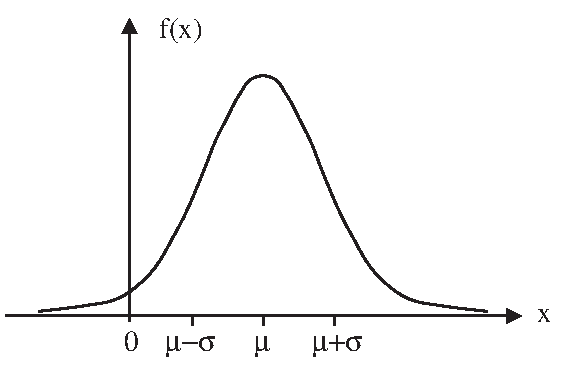
\includegraphics[scale=1.0]{figurer/fig8_5.pdf} 
 \caption{Normalfordelingen $N(\mu , \sigma ^2)$}
	\label{fig:Normalfordelingen}
\end{figure}
Kurven er bestemt ved funksjonen
\[   f(x)=\frac{1}{\sqrt{2\pi}\sigma} e^{-\frac{1}{2\sigma^2}(x-\mu )^2} \]
og alle sannsynligheter i forbindelse med $X$ kan finnes ved
å beregne arealer under denne kurven. Som vi har sett kan
dette alltid føres tilbake til å beregne arealer under
normalkurven $g(z)$. Denne svarer til $N(0,1)$, dvs.
normalfordelingen med forventning $0$ og varians $1$, den
såkalte {\em standardnormalfordelingen}.

I fagterminologien blir $f(x)$ kalt {\em sannsynlighetstettheten}
til $X$. Generelt for slike gjelder at de er ikke-negative og
avgrenser et totalt areal lik $1$. En kontinuerlig
sannsynlighetsmodell er en modell som kan beskrives ved en
sannsynlighetstetthet og der sannsynligheter er gitt ved arealer
under tettheten. For regning med kontinuerlige modeller trengs
ferdighet i inte\-gralregning, eksempelvis er 

\[  P(a\le X \le b)=\int\limits_a^b f(x)dx \]
og forventningen til $X$ er definert ved

\[EX=\int \limits_{-\infty}^{\infty} x f(x)dx \]
I forbindelse med normalfordelte variable kan det vises en rekke
setninger, spesielt viktig er denne:

\begin{center} \framebox[10cm]{\begin{minipage}{9cm}\rule{0cm}{0.5cm}
En stokastisk variabel som kan skrives som en lineær funksjon
av uavhengige normalfordelte variable  er selv normalfordelt.\\
\mbox{} \end{minipage}}  \end{center}
Dette har en rekke viktige konsekvenser bl.a.:

For målemodellen: Dersom vi føyer til en antakelse om at
observasjonene $X_1,X_2,\ldots ,X_n$ alle er normalfordelte,
medfører dette at $\bar X$, som er en lineær funksjon av
observasjonene, også er normalfordelt, med forventning $\mu$
og varians $\sigma ^2/n$. 

For regresjonsmodellen: Dersom vi føyer til en antakelse om at
observasjonene $X_1,X_2,\ldots ,X_n$ alle er normalfordelte,
medfører dette at $\hat\alpha$ og $\hat\beta$, som begge er
lineære funksjoner av observasjonene, også er
normalfordelt, med forventninger $\alpha$ og $\beta$ og varianser
henholdsvis $\sigma ^2/n$ og $\sigma ^2/M$.

Dette betyr at i en målemodell eller en regresjonsmodell hvor
normalitet inngår som en av forutsetningene i modellen, vil de
sannsynlighetsutsagn som ble etablert i avsnittene 8.1 og 8.3 som
tilnærmede utsagn, være å oppfatte som eksakte. Dette
gjelder for de problemstillinger der variansen til observasjonene
$\sigma ^2$ er kjent. Mer oppsiktsvekkende er at det er mulig
å etablere eksakte sannsynlighetsutsagn i
situasjoner der $\sigma ^2$ er ukjent og må estimeres på
grunnlag av observasjonene. La oss utdype dette:

I målemodellen med normalitetsantakelse vil den stokastiske
variable

     \[Z={\bar X - \mu \over \sigma (\bar X)}={\bar X -\mu
     \over \sigma/ \sqrt n}\]
være en nøkkelstørrelse i forbindelse med inferens om
$\mu$. Den vil være fordelt $N(0,1)$ og danner i situasjoner
der $\sigma$ er kjent et utgangspunkt for konstruksjon av
sannsynlighetsutsagn. Dersom $\sigma$ er ukjent er $Z$ ubrukelig
til dette. Man kan isteden ta utgangspunkt i den stokastiske variable 

\[T=\frac{\bar X - \mu}{S(\bar X)}=\frac{\bar X -\mu}{S/ \sqrt{n}}\]
dvs. en analogi til $Z$ der $\sigma$ er erstattet med en
estimator $S$. Det har vært vanlig å bruke $S=\sqrt{S^2}$ der

\[   S^2={1\over n-1} \sum_{i=1}^n (X_i -\bar X)^2\]
som er en forventningsrett estimator for $\sigma ^2$ i
målemodellen. I regresjonsmodellen med normalitetsantakelse
vil den stokastiske variable

\[  Z=\frac{\hat{\beta}-\beta}{\sigma (\hat{\beta})}=
       \frac{\hat{\beta} - \beta}{\sigma /\sqrt M}\]
være fordelt $N(0,1)$ og danner i situasjoner der $\sigma$ er
kjent et utgangspunkt for konstruksjon av sannsynlighetsutsagn
ved inferens om $\beta$. Dersom $\sigma$ er ukjent kan man
isteden ta utgangspunkt i

\[T={\hat{\beta} -\beta \over S(\hat\beta)}={\hat\beta -
                                     \beta\over S/ \sqrt{M}}\]
dvs. $\sigma$ er erstattet med en estimator $S$. Det er vanlig
å bruke $S=\sqrt{S^2}$ der

\[S^2={1\over n-2} \sum_{i=1}^n (X_i -\hat\alpha-
                              \hat\beta(t_i -\bar t))^2\]
som er en forventningsrett estimator for $\sigma ^2$ i
regresjonsmodellen.

Dersom vi kjente sannsynlighetsfordelingen
til $T$ i situasjonene ovenfor, kunne vi bruke $T$ til å lage
sannsynlighetsutsagn på tilsvarende måte som med $Z$ i
situasjonen med $\sigma$ kjent.  Under forutsetning av at observasjonene
i modellen er normalfordelte kan det vises at $T$, i begge situasjoner,
har en kontinuerlig modellkurve som er klokkeformet og
symmetrisk om null, en såkalt t-kurve. Den ligner 
normalkurven, men har noe tyngre ``haler" enn denne, se Figur~\ref{fig:t_kurve}.

\begin{figure}[ht]
\centering
	\includegraphics[scale=1.0]{figurer/fig8_6.pdf} 
 \caption{t-kurve og normalkurve}
	\label{fig:t_kurve}
\end{figure}
Det matematiske uttrykk for t-kurven er relativt komplisert og
utelates her. Kurvens eksakte form vil avhenge av $n$, med
svært tunge haler for liten $n$ og mer og mer lik
normalkurven ettersom $n$ vokser. Dette lar seg forklare ved at
når $\sigma$ blir erstattet med $S$ vil dette være årsak 
til større risiko for verdier fjernt fra symmetripunktet, men
når $n$ er stor vil $S$ gi et meget presist anslag for
$\sigma$, slik at det spiller mindre rolle om $\sigma$ er
erstattet med $S$.

I målemodellen brukes den såkalte t-fordeling med $n-1$
frihetsgrader, i regresjons\-modellen t-fordelingen ned $n-2$
frihetsgrader. Frihetsgradtallet uttrykker da graden av
usikkerhet som skyldes at $\sigma$ er estimert: stort
frihetsgradtall, liten usikkerhet.

Arealer under t-kurver er
tabellert og er lett tilgjengelig i tabellverker. Slike tabeller
kan, i situasjoner der $\sigma$ er ukjent, brukes på samme
måte som vi har brukt arealer under normalkurven i
situasjonen med kjent varians. Siden det trengs en t-tabell for
hvert frihetsgradtall, er t-tabellene vanligvis mindre detaljerte
enn de tilsvarende normaltabeller. Vanligvis gis punkter som
avgrenser bestemte arealer til høyre eller venstre for seg,
såkalte fraktiltabeller, se Tabell~\ref{tab:T_kurver_Fraktil} i Appendiks~\ref{app:fordelngstabeller}. 
Med andre ord har vi at

\[  P(Z\le k)=G(k) \mbox{\ \ \ mens\ \ \ } P(T\le k)=G_m(k)  \] 
der $G_m(k)$ betegner arealet til venstre for $k$ under t-kurven
med $m$ frihetsgrader, med $m=n-1$ for målemodellen og $m=n-2$
for regresjonsmodellen. Videre er

\[  P(\mid Z \mid \le k)=A(k) \mbox{\ \ \ mens\ \ \ }P(\mid T \mid \le k)=A_m(k)\]
der $A_m(k)$ betegner arealet mellom $-k$ og $k$ under t-kurven.
På grunn av symmetrien har vi som i tilfellet med normalkurven at 
                                 
\[     A_m(k)=2G_m(k)-1\]
For målemodellen betyr dette at

\[   P(\mid\bar X -\mu\mid \le k\cdot S(\bar X))=A_{n-1}(k)\]
dvs. vi kan i prinsippet konstruere eksakte sannsynlighetsutsagn
vedrørende $\bar X$ som estimator for $\mu$ av typen:
Sannsynligheten for at $\bar X$ avviker fra $\mu$ med høyst
$k$ ganger anslått standardavvik er $A_{n-1}(k)$. For
regresjons\-modellen gjelder tilsvarende at

\[ P(\mid\hat\beta -\beta\mid\le k\cdot S(\hat\beta))=A_{n-2}(k).\]
Her er det også mulig å lage sannsynlighetsutsagn om
estimeringsfeilen ved $\hat X$ som estimator for forventet
respons $EX=\gamma+\beta t$ for en gitt $t$. Vi har nemlig

\[ P(\mid\hat X -(\gamma +\beta t)\mid \le k\cdot S(\hat X))=A_{n-2}(k)\]
Endelig er det mulig å lage sannsynlighetsutsagn om prediksjonsfeilen ved 
å bruke $\hat X$ som prediktor for en ny observasjon $X$ for 
gitt $t$:

\[ P(\mid \hat X - X\mid \le k\cdot S(\hat X -X))=A_{n-2}(k)\]
I disse formlene inngår estimerte standardavvik for hhv. prediktor og
prediksjonsfeil, jfr. Oppgave~35.
\begin{eqnarray*}
 S(\hat{X})&=&S\cdot \sqrt{\frac{1}{n}+ \frac{(t-\bar t)^2}{M}} \\
 S(\hat{X}-X)&=&S\cdot \sqrt{1 + \frac{1}{n}+ \frac{(t-\bar t)^2}{M}}
\end{eqnarray*}
Merk at begge avhenger av $t$, og
øker ettersom $t$ avviker mer og mer fra $\bar t$.

Vi har altså konstatert at antakelse om normalitet åpner
nye muligheter, men under hvilke omstendigheter vil en
normalitetsantakelse i tillegg til de andre antakelsene i en
modell være realistisk? I praksis finner vi to typer
argumenter. Enten brukes et teoretisk argument om at verdien av
hver stokastisk variabel i modellen er bestemt av en rekke
faktorer som virker uavhengig av hverandre, og en referanse til
sentralgrensesetningen støtter da opp om en
normalitetsantakelse. Eksempelvis kan høyden til en utvalgt
16-åring tenkes å være bestemt av en rekke
arvemessige og miljømessige faktorer som summeres opp.
Alternativt brukes et empirisk argument om at praktisk erfaring
fra lignende situasjoner har vist at den
sannsynlighetsfordeling det er tale om har klokkefasong som til
forveksling ligner normalfordelingen. Hvorfor ikke uttrykke
slik forhåndsviten eksplisitt i modellen?

I mange situasjoner er det imidlertid ikke rimelig å trekke
veksler på noen av disse argumentene, og da bør en
selvsagt ikke inkludere normalitet blant forutsetningene i
modellen. I praksis ser en dessverre ofte benyttet metoder som
forutsetter normalitet uten at dette rettferdiggjøres, ja
endog er brukeren bevisst. Det finnes metoder til å sjekke om
et tallmateriale med rimelighet kan sies å være generert
av en normalfordeling.

La oss nå kommentere visse optimale egenskaper ved de metoder
som er foreslått i Kapittel 8.1 og 8.3, og deretter komme med
visse reservasjoner:

For estimering av forventningen $\mu$ i målemodellen kan det
vises at estimatoren $\bar X$ har følgende egenskaper:
\begin{enumerate}
\item $\bar X$ er den forventningsrette estimator for $\mu$ som har
minst varians blant de forventningsrette estimatorer som er
lineære funksjoner av observasjonene $X_1,X_2,\ldots ,X_n$
(Gauss-Markov's setning).
\item $\bar X$ er den forventningsrette estimator $\mu$ som har
minst varians dersom vi er villig til å anta at
sannsynlighetsfordelingen til observasjonene er normal.
\end{enumerate}
Vi kan imidlertid innvende: Under 1. begrenser en seg til klassen
av lineære forventningsrette estimatorer. Kan hende finnes
det en estimator utenfor denne klassen som er bedre. Under 2.
antas det at observasjonene har en såkalt normalfordeling.
Kan hende dette er en urealistisk antakelse.

Det finnes også teoretiske resultater som sier at ved testing
av hypoteser om $\mu$ i målemodellen, så vil testmetoder
basert på $\bar X$ være optimale i en viss forstand.
Videre finnes teori som sier at ved estimering og testing i den
enkle regresjonsmodellen, så vil metoder basert på
$\hat\alpha$ og $\hat\beta$ slik de er definert i Kapittel 8.3
være optimale i en viss forstand.
                                                              
Med utgangspunkt i de ideer som er skissert ovenfor er det med
årene utviklet omfattende generell teori basert på forutsetninger
om normalitet (og ukjent varians), bl.a. teorien for lineære
normale modeller som i dag regnes som klassisk statistisk
teori.\footnote{Som grunnlegger av denne teori regnes Ronald A.
Fisher (1890-1962).} Videre er det utviklet brukerorienterte
spesialområder såsom variansanalyse og regresjonsanalyse,
se Kapittel 11 og 12. 

\section{ Mer om måleproblemer}

Ved de fleste praktiske anvendelser av målemodellen, vil nok
variansen til observasjonene være ukjent. Dersom vi kan
rettferdiggjøre at observasjonene er normalfordelte, vil en
kunne dra nytte av teorien i forrige avsnitt til å konstruere
konfidensgrenser og tester med eksakte sikkerhetsgarantier, selv
når antall observasjoner er lite. Bruker vi metoder basert
på modeller der variansen er kjent, forutsetter vi egentlig
at vi allerede har anslått denne i en lignende situasjon, med
et stort antall observasjoner som grenser til sikkerhet, og at vi
er villig til å anta at variabiliteten er den samme i den
foreliggende situasjon.

Dette kan være en betenkelig
praksis, fordi omstendighetene kan være endret uten at vi er
klare over det. En varians som i modellen er gitt en urealistisk verdi,
kan føre til feiltolkning av tallmaterialet. For å
unngå dette er det anbefalt at variansen anslås ut fra
tallmaterialet selv, også når det foreligger betydelig
forhåndsinformasjon.
I målemodellen med normalitetsantakelse om observasjonene
bestemmer

\[  \bar X \pm k\cdot S(\bar X)\]
et konfidensintervall for forventningen $\mu$ med
konfidensnivå $c=A_{n-1}(k)$ (arealet mellom $-k$ og $k$ under t-
kurven med $n-1$ frihetsgrader). Ønsker vi å teste
hypotesen $H_0:\mu={\mu}_0$ mot en alternativ hypotese, kan vi
bruke den såkalte $t$-observatoren

\[    T=\frac{\bar{X}- {\mu}_0}{S(\bar{X})}\]
som, dersom $H_0$ er riktig, er $t$-fordelt med $n-1$
frihetsgrader. Forkastningsområdet og bestemmelse av kritisk
verdi avhenger av den alternative hypotesen, likeledes eventuell
beregning av $P$-verdi. Vi har i hovedsak tre tilfeller:
\begin{center}
\begin{tabular}{cccl}
Tilfelle  & Alternativ  &   Forkastningsområde &  $P$-verdi \\ \hline
a. & $\mu< {\mu}_0$     &    $T\le k$         &   $P_{H_0}(T\le t)$\\
b. & $\mu > {\mu}_0 $   &    $T\ge k$         &   $P_{H_0}(T\ge t)$ \\
c. & $\mu \ne {\mu}_0$  &   $\mid T\mid \ge k$&$P_{H_0}(\mid T\mid \ge t)$\\ \hline 
\end{tabular}
\end{center}
Den kritiske verdi $k$ bestemmes slik at arealet under t-kurven
svarende til forkastningsområdet er lik det ønskede
signifikansnivå, se Figur~\ref{fig:krit_verdi_t}a-c.

\begin{figure}[ht]
\centering
	 \includegraphics[scale=0.6]{figurer/fig8_7.pdf} 
 \caption{Kritiske verdier for t-testen}
	\label{fig:krit_verdi_t}
\end{figure}
Vi husker at et konfidensintervall kan tolkes som mengden av
plausible verdier av $\mu$. I tilfellet c der alternativet er
tosidig, kan en alternativt bruke konfidensintervallet ved
hypotesetesting. Dersom nullhypotesen faller utenfor
konfidensgrensene forkastes hypotesen. Dette er ekvivalent med $t$-
testen med signifikansnivå $\alpha =1-c$, der $c$ er
konfidensnivået. Vi kan også bruke konfidensgrensene
når alternativet er ensidig. Da forkastes hypotesen når
denne er utenfor den relevante konfidensgrensen (den øvre i
tilfelle a og nedre tilfelle b). I det tilfellet er
signifikansnivået isteden $\alpha=(1-c)/2$, dvs. $c=1-2\alpha$.\\

\begin{eksempel}{Forurensing}
La situasjonen være som i Eksempel 3, med følgende
observerte verdier av kvikksølvkonsentrasjonen
\begin{center}
\begin{tabular}{ccccccccc}
     14.8 & 15.4 & 16.1 & 14.7 & 17.5 & 15.9 & 13.4 & 16.0 & 15.7
\end{tabular}
\end{center}
Vi finner at $\bar{X}$=15.5, $S$=1.138, slik at $S(\bar{X})=S/\sqrt{9}=0.38$.
Antas observasjonene normalfordelte vil eksakte
konfidensintervaller for forventet konsentrasjon $\mu$ ha form

\[ 15.50\; \; \pm \; \; k\cdot 0.38\] 
der sikkerhetsfaktoren $k$ finnes i Tabell~\ref{tab:T_kurver_Fraktil} med frihetsgradtall
$\nu =9-1=8$ og det ønskede konfidensnivå. Eksempelvis
krever konfidensnivået 0.95 at $k=2.31$, mens $k=1.96$ var
nok i tilfellet med kjent varians. Konfidens\-nivået lik 0.90 krever
$k=1.86$, mot $k=1.645$ i tilfellet med kjent varians, se Oppgave~2.
La oss se på en typisk $t$-analyseutskrift:\\
\begin{center} \framebox[10cm]{\begin{minipage}{9cm}\rule{0cm}{0.5cm}
\tt               
 >> READ 'eks8.7' X\\
 >> TINTERVAL 0.90 X \\
\begin{tabular}{lrrrrc}
       &      N &    Mean &  StDev & SeMean & 90.0 \% ConfInt\\
 X     &      9 &  15.500 &  1.138 &  0.379  & ( 14.79, 16.21 )
 \end{tabular} \\
 >> TTEST 17.2 X \\
  Test of MU = 17.200 vs MU not = 17.200\\
 \begin{tabular}{lrrrrrr}
        &    N  &   Mean  & StDev  & SeMean  &   T   & P-value \\
 X      &    9  & 15.500  & 1.138  &   0.379  & -4.48 &  0.0021
 \end{tabular} \\
\end{minipage}} \end{center}
Her er data lest fra en fil 'eks8.7' og lagret som en søyle $X$.
Vi ber om et konfidensintervall med konfidens\-nivå  0.90, som gir
intervallet [14.79, 16.21], i tillegg til de beskrivende mål.
Her er\\[1mm]
\noindent  Mean=gjennomsnittet av observasjonene \\
StDev=standardavviket til observasjonene  \\
SeMean=anslått standardavvik til gjennomsnittet (ofte kalt standardfeilen).\\
Leseren kan selv sjekke at beregningen samsvarer med teorien ovenfor.
Videre ber vi om å få utført en $t$-test av hypotesen $\mu =17.20$,
og får, i tillegg til de beskrivende mål, beregnet $T$ og 
$P$-verdien. Med 5\% nivå forkastes hypotesen ($P<0.05)$. 
Dersom bare en eventuell reduksjon i kvikk\-sølv\-konsen\-trasjonen
er aktuell eller ønskes fastslått, slik at alternativet til
nullhypotesen er ensidig, må den oppgitte $P$-verdi halveres, dvs.
$P=0.00105$. Programvare gir vanligvis anledning til å spesifisere dette.

Egen kommando for $t$-test er egentlig unødvendig,
idet vi kan sjekke om nullhypotesen ligger i $t$-intervallet eller ikke.
Konfidensnivå 90\% svarer til 10\% signifikansnivå i det tosidige
tilfellet og 5\% i det ensidige tilfellet.
\end{eksempel}

Planlegging av antall observasjoner i forbindelse med $T$-metoder
krever betydelig mer kompliserte regninger enn tilfellet var for
de tilsvarende $Z$-metodene. Grove betraktninger med antatt kjent
varians kan likevel være til noen hjelp, men statistiske
programpakker bør kunne gi støtte her. Hittil har dette
aspekt vært neglisert i de fleste pakker, men den følge at
 $t$-intervaller og $t$-testen misbrukes i betydelig grad i praksis.
Ukritisk bruk av konfidensintervaller med konvensjonelle
konfidensnivåer $(90\%, 95\%,99\%)$ innebærer ofte en
ensidig fokusering på sikkerheten på bekostning av
presisjonen (konfidensintervallets lengde), og neglisjering av
planleggingsfasen. Anvendt i forkast-aksept situasjoner
innebærer dette en neglisjering av risikoen for akseptfeil.
Ukritisk hypotesetesting med konvensjonelle signifikansnivåer
eller beregning av $P$-verdier, innebærer ofte at risikoen for
godtakingsfeil i forbindelse med vesentlige avvik fra
nullhypotesen ikke er vurdert, igjen et
planleggingsspørsmål. 
                               
Det hender ofte at en er usikker på om forutsetningene for
bruk av målemodellen er oppfylt, og en kan ønske seg
metoder som forsøker å stille en diagnose ut fra
observasjonene selv. Forutsetningene var:  $(i)$ samme forventning
$(ii)$ samme varians $(iii)$ uavhengighet og eventuelt $(iv)$
normalitet. Det finnes formelle metoder der hver forutsetning tas
som en nullhypotese, og der en tilhørende test er egnet til
å avsløre spesielle alternativer til denne. Vi vil ikke
gå inn på slike metoder her, men heller antyde bruken av
mer uformelle grafiske metoder, sammen med en viss intuisjon.
Ofte kan brudd på forutsetningene $(i) - (iii)$ avsløres
ved å se på observasjonene gruppevis hvis de er tatt
på ulikt tidspunkt, ulikt sted eller av ulike personer.
Dersom det er en naturlig rekkefølge av observasjonene er det
lurt å plotte dem som funksjon av observasjonsnummeret.
Eksempler på dette gis i Figur~\ref{fig:diagnoseplott}a-f.

\begin{figure}[H]
\centering
	 \includegraphics[scale=0.8]{figurer/fig8_8.pdf} 
 \caption{Diagnose-plott}
	\label{fig:diagnoseplott}
\end{figure}
I Figur~\ref{fig:diagnoseplott}a ser observasjonene ut til å variere tilfeldig
omkring en forventning markert med den  horisontale linje, og at
(i) - (iii) er oppfylt. I Figur~\ref{fig:diagnoseplott}b ser observasjonene ut til
å falle i to grupper med ulik forventning, slik at (i) ikke
er oppfylt, men (ii) godt kan være det. Teori for denne
situasjonen finnes i Kapittel 11. I Figur~\ref{fig:diagnoseplott}c ser det ut til at
forventningen øker med observasjonsnummeret, men at (ii) og
(iii) godt kan være oppfylt. Dette innbyr til en
regresjonsmodell, dersom det er meningsfylt. I Figur~\ref{fig:diagnoseplott}d ser det
ut til at variansen øker, slik at (ii) ikke er oppfylt. I
Figur~\ref{fig:diagnoseplott}e ser det ut til at etterfølgende observasjoner er
korrelerte, slik at (iii) ikke er oppfylt. Teori for denne
situasjon finnes i Kapittel 13. Figur~\ref{fig:diagnoseplott}f antyder en ``vill"
observasjon som bryter med forutsetningen om normalitet, og som
eventuelt må korrigeres eller fjernes før $t$-metoden
brukes.

En indikasjon på om normalitet $(iv)$ er en rimelig
antakelse, får vi ved å gruppere observasjonene, og lage
et histogram, se Figur 1.2 i Eksempel 1.6. Det kan imidlertid
være vanskelig å skille en normalfordeling fra andre
symmetriske fordelinger. For dette formål kan derfor et
såkalt normalskår-plott være et hensiktsmessig
diagnoseredskap. De $n$ observasjonene $X_1,X_2,\ldots ,X_n$
ordnes først i stigende rekkefølge. Den i'te observasjon
talt nedenfra, kall den $X_{(i)}$, tildeles så en såkalt
normalskår $Y_{(i)}$ bestemt ved \footnote{Noen statistiske
programpakker med innlagt normalskårfunksjon bytter om de to aksene, og
bruker kanskje en annen likeverdig definisjon.} 

\[     G(Y_{(i)})=\frac{i}{n+1} \mbox{\ \ \ }   i=1,2,\ldots ,n\]
Vi har da bestemt en normalskår $Y_i$ til hver observasjon
$X_i$, og vi kan plotte tallparet $(X_i,Y_i)$ for
$i=1,2,\ldots ,n$ i et spredningsdiagram. Dersom
den observerte fordeling av $X_i$'ene kan tilnærmes med en
normalfordeling, vil punktene i normalskårplottet ligge
noenlunde på linje. Figur~\ref{fig:avvik_normalitet}a-c illu\-strerer formen på
plottet for noen typiske avvik fra normalitet. Dersom den
observerte fordeling er symmetrisk, men har ``tyngre haler" enn
normalfordeling, vil punktene anta en S-form (Figur~\ref{fig:avvik_normalitet}a), mens ved
``lettere haler" enn normalfordelingen, vil punktene anta en
omvendt S (Figur~\ref{fig:avvik_normalitet}b). Dersom den observerte fordeling er skjev
med lang hale mot høyre, vil plottet ha form som i Figur~\ref{fig:avvik_normalitet}c.

\begin{figure}[H]
\centering
	 \includegraphics[scale=0.7]{figurer/fig8_9.pdf} 
 \caption{Avvik fra normalitet}
	\label{fig:avvik_normalitet}
\end{figure}
Nå vil, som vi har antydet ovenfor, normalitet kunne være
en urea\-listisk antakelse, men man trodde lenge at de metodene som
hadde vist seg å være optimale under
normalitetsantakelser, også var uten alvorlige konkurrenter i
situasjoner der den underliggende 
sannsynlighetsfordeling ikke nødvendigvis var normal. Dette
viste seg ikke alltid å være tilfellet. I de senere
tiår har statistikerne derfor i stigende grad rettet
oppmerksomheten mot en rekke alternative metoder, såkalte
{\em robuste metoder}. Disse har den egenskapen at dersom den
underliggende fordeling virkelig er normal så taper en noe,
men ikke mye, i forhold til de ``optimale" metodene, mens på
den annen side kan gevinsten være betydelig dersom
fordelingen avviker noe fra normalfordelingen.

La oss i forbindelse med målemodellen kort antyde en
situasjon hvor estimatoren $\bar X$ får alvorlige
konkurrenter. Anta at det er en viss sjanse for ``ville "
observasjoner, dvs. verdier langt fra den $\mu$ vi skal estimere.
I et gjennomsnitt hvor alle observasjonene er gitt samme vekt,
vil en ``vill" verdi lett kunne ødelegge den tendens som de
andre observasjonene samlet gir. En mulig måte å redusere
virkningen av ville observasjoner, er å ordne observasjonene i
stigende rekkefølge, stryke den minste og den største
observasjonen, og ta gjennomsnittet av de resterende $n-2$
observasjonene. Mer generelt kunne vi stryke de $k$ minste og de
$k$ største observasjonene og ta gjennomsnittet av de
resterende. Et slikt gjennomsnitt kalles et {\em trimmet
gjennomsnitt}. Den mest ekstreme form for trimming får vi
når vi stryker alle observasjonene unntagen den midterste
(evt. de to miderste). Vi sitter da igjen med den såkalte
{\em medianen} av observasjonene. Det kan vises at i visse situasjoner
vil medianen være å foretrekke framfor alle andre
estimatorer. I Eksempel 1 ser vi at medianen av observasjonene er
$0.65$, mens i Eksempel 2 er medianen $9.725$. Dersom man i en gitt
situasjon velger å rapportere medianen (eller et annet
trimmet gjennomsnitt) bør også dette følges av
(estimert) standardavvik.

Formler for standardavvik til trimmede gjennomsnitt er ofte
kompli\-serte, vanskelig å utlede, og avhenger typisk av den
underliggende fordeling. Det fins en alternativ tilnærming,
som gjør det mulig å anslå standardavvik i ikke-standard
 situasjoner, uten å kjenne de fordelingsteoretiske egenskapene
i detalj. Metoden kalles {\em resampling}, og er blitt
mulig først med dagens raske regneteknologi.
En kort beskrivelse er gitt i avsnitt 8.7. 

\section{Mer om regresjonsproblemer}
I de fleste praktiske situasjoner der en foretar statistiske
analyser basert på en regresjonsmodell, er det lite rimelig
å anta at variansen til observasjonene er kjent. Dersom vi er
villige til å anta at observasjonene er normalfordelte, vil
derfor teorien i Kapittel 8.4 kunne hjelpe oss et stykke videre.
Mange av dagens regresjonsanalyseprogrammer gir også
utskrifter hvor fortolkningen i betydelig grad er knyttet til
normalitetsantakelsen. 

I regresjonsmodellen med normalitetsantakelse om observasjonene gir

\[      \hat{\beta} \;\; \pm \;\; k\cdot S(\hat{\beta})\]
et konfindensintervall for regresjonskoeffisienten $\beta$ med
konfidensnivå $c=A_{n-2}(k)$, dvs. lik arealet mellom $-k$ og $k$
under $t$-kurven med $n-2$ frihetsgrader. Ønsker vi å teste hypotesen
$H_0:\beta ={\beta}_0$ mot en alternativ hypotese kan vi bruke $t$-
observatoren

\[   T=\frac{\hat{\beta}-{\beta_0}}{S(\hat{\beta})}\]
som, dersom $H_0$ er riktig, er $t$-fordelt med $n-2$
frihetsgrader. Forkastningsområdet og bestemmelse av kritisk
verdi avhenger av den alternative hypotesen, likeledes beregning
av $P$-verdi. Vi kan bruke den samme skjematiske oppstilling og
figurer som for målemodellen i forrige avsnitt. I noen
situasjoner er det aktuelt å lage konfidensintervaller og
teste hypoteser om konstantleddet. Dette kan gjøres på
tilsvarende måte som for regresjons\-koeffisienten. Resultatene
i Kapittel 8.4. gir videre at

\[   \hat{X} \;\; \pm \;\; k\cdot S(\hat{X})\]
er et konfidensintervall for forventningen $EX$ for en gitt $t$, mens 

\[   \hat{X} \;\; \pm \;\; k\cdot S(\hat{X}-X)\]
er et såkalt prediksjonsintervall for en ny uavhengig
observasjon for en gitt $t$.  Sikkerhetsfaktoren $k$ bestemmes i
begge tilfeller slik at arealet mellom $-k$ og $k$ under $t$-kurven
med $n-2$ frihetsgrader er lik det ønskede konfidensnivå.
Regresjonsanalyseprogrammer vil som regel kunne utføre
beregningen av ønskede estimerte standardavvik, enten
automatisk eller som en opsjon, slik at formlene fra Kapittel
8.4. kan unngås. 
Merk imidlertid at

\[ S(\hat X - X)=\sqrt{S^2+(S(\hat X))^2}\]
som gir mulighet for å beregne den tredje størrelsen
straks de to øvrige er kjente.\\

\begin{eksempel}{Aktivitet - Avfall}
Konsentrasjonen av et avfallsstoff i en elv måles
regelmessig. I tillegg til en viss ``naturlig" konsentrasjon
kommer avfallet fra en bedrift, og forventet bidrag fra denne
antas i hvert fall ikke å avta med aktivitetsnivået. Følgende
observasjoner på 12 ulike tidspunkter foreligger:
\begin{center}\small \addtolength{\tabcolsep}{-0.4\tabcolsep}
\begin{tabular}{lcccccccccccc}
Aktivitetsnivå $(t)$:& 3 & 5 & 2 & 4 & 2 & 1 & 3 & 1 & 2 & 5 & 4 & 3\\    
Konsentrasjon $(X)$ :&    4.7&6.4&3.5&5.4&3.9&2.6&5.9&4.1&5.1&4.6&6.1&3.0
\end{tabular}
\end{center}
Spredningsdiagrammet for observasjonene ser ut som i Figur~\ref{fig:Spredningsdiagram}.

\begin{figure}[H]
\centering
	 \includegraphics[scale=0.7]{figurer/fig8_x.pdf} 
 \caption{Spredningsdiagram}
	\label{fig:Spredningsdiagram}
\end{figure}
En utskrift fra et analyseprogram for lineær regresjon gir typisk:

\begin{center} \framebox[11cm]{\begin{minipage}{10cm}\rule{0cm}{0.5cm}
\tt
 >> READ 'eks8.8' t X \\
\  >> REGRESS  X ON t\\
  X = 2.91 + 0.584 t (S=0.9728)\\
 \begin{tabular}{rrrrr}
            &           &   St.Dev. & T-ratio=&        \\
 Variable   &Coefficient&  of Coef. & Coef/S.D&      P \\
            &  2.9060   &   0.6810  &    4.27 &  0.002 \\
       X    &  0.5837   &   0.2127  &    2.74 &  0.021
 \end{tabular} \\
Degrees of Freedom for T-test = 10\\
R-squared = 43.0\% (Adjusted for d.f. = 37.2\%)\\
\mbox{}
\end{minipage}} \end{center}

Vi ser at regresjonskoeffisienten på 0.5837 er såpass stor i forhold
til sitt anslåtte standardavvik på 0.2127, at det er grunn til
å hevde at konsentrasjonen øker med aktivitetsnivået i bedriften.
Med 10 frihetsgrader blir nødvendig sikkerhetsfaktor svarende til
95 \% konfidensnivå lik $k$=2.228, som gir konfidensintervallet
 $0.5837 \pm 2.228 \cdot 0.2127$, dvs. [0.110 , 1.058]. Intervallet omfatter ikke null.

Merk at de $T$-verdier som skrives ut svarer til nullhypotesen at
koef\-fisienten er null, og at $P$-verdi er gitt for tosidig alternativ.
 $P$-verdien for situasjoner med  ensidig alternativ er halvparten, i vår
situasjon blir det 0.0105. Dette betyr at med valgt signifikansnivå på
5\%, vil nullhypotesen bli forkastet, men ikke dersom signifikansnivået er
valgt lik 1\%.
Dersom nullhypotesen skulle være noe annet enn null, er vi nødt
til å regne ut $T$-brøken selv, og slå opp $P$-verdi i tabell.

Estimert standardavvik omkring regresjonslinjen ser vi er $S=0.9728$, som gir en
grov indikasjon på typiske prediksjonsfeil ved å bruke 
regresjons\-linjen som
prediktor. Utskriften inneholder også  opplysninger om hvor stor del av
variasjonen i konsentrasjonen av avfall som blir forklart ved
variasjonen i aktivitetsnivået ($R$-squared). Dette blir 
forklart nærmere i Kapittel 12.

Et regresjonsprogram vil som regel kunne gi mer detaljerte opplysninger
om bruken av $\hat X$ som estimator eller prediktor for gitt $t$ :\\

\begin{center} \framebox[11cm]{\begin{minipage}{10cm}\rule{0cm}{0.5cm}
\tt
>> PREDICT X for t=1 2 3 4 5\\
\addtolength{\tabcolsep}{-0.2\tabcolsep}
\begin{tabular}{cccccc}
    &        &   StD &  StD   &   Conf.Int.&  Pred.Int.  \\
 t  &   Fit  &   Fit & PredErr& 95\%   & 95\% \\
 1  & 3.490  &  0.495  & 1.091 & (2.386,4.593) & (1.057,5.922)  \\ 
 2  & 4.073  &  0.342  & 1.031 & (3.311,4.835) & (1.775,6.371)   \\
 3  & 4.657  &  0.281  & 1.013 & (4.030,5.284) & (2.400,6.914)   \\
 4  & 5.241  &  0.363  & 1.038 & (4.431,6.050) & (2.926,7.555)   \\
 5  & 5.824  &  0.525  & 1.105 & (4.655,6.994) & (3.361,8.288)   
\end{tabular}
\end{minipage}} \end{center}
 
\noindent Her er gitt estimater/prediksjoner for aktivitetsnivåene 
1, 2, 3, 4, 5, med tilhørende standardavvik for henholdsvis estimat og
prediksjonsfeil. I tillegg gis konfidensintervaller for forventet
konsentrasjon og prediksjonsintervaller for ny observerbar konsentrasjon 
svarende til 95\% sikkerhet, som fortsatt er beregnet på grunnlag av
sikkerhetsfaktoren $k$=2.228 for tilfellet med 10 frihetsgrader. 
Leseren kan selv sjekke beregningen, samt beregne tilsvarende
intervaller for andre sikkerhetsnivåer.

Merk at dersom programmet ikke gir
annet enn $\hat X_i$ og $S(\hat X_i)$, kan de øvrige
størrelser beregnes enkelt ved formlene ovenfor.
\end{eksempel}

Bruken av t-tabellen er i dette eksemplet knyttet til en
regresjonsmodell med normalfordelte observasjoner. Selv om
spredningsdiagrammet gir en viss pekepinn på om de ulike
forutsetningene er oppfylt, kan vi ønske oss ytterligere
hjelpemidler til å sjekke disse. Sentralt her er de
observerte {\em residualene}, som er de enkelte observasjonenes vertikale avstand
fra den estimerte regresjonslinjen. Vi skriver

\[   \hat U_i=X_i - \hat X_i \mbox{\ \ \ } i=1,2,\ldots ,n\]
Disse kan oppfattes som ``observasjoner" av de forventede avvik
$U_i=X_i - EX_i$, $i=1,2,\ldots ,n$, som, under forutsetningene i
regresjonsmodellen: $(i)$ har samme forventning lik null $(ii)$
har samme varians $(iii)$ er uavhengige  og $(iv)$ er
normalfordelte.

Ulike former for plott av de observerte
residualene vil kunne avsløre avvik i disse forutsetningene.
En kan plotte residualene som funksjon av observasjonsnummeret,
og de samme betraktninger som i Kapittel 8.5 kan gjøres, jfr.
Figur~\ref{fig:diagnoseplott}a-f. Alternativt kan en plotte residualene mot
høyresidevariablen $t$.

Ved vurdering av unormalt store
residualer, må disse ses i forhold til sitt standardavvik.
Siden $S$ estimerer standardavviket $\sigma$ til de sanne
resi\-dualene, kan en se de observerte residualer i forhold til
$S$. Det viser seg imidlertid at standardavviket til de
observerte residualene avhenger av $n$ og $t$, og er mindre enn
$\sigma$. For ikke å undervurdere residualene mht. avvik, bør
standardavviket til de observerte residualene estimeres med
\footnote{Til forskjell fra formelen for estimert standardavvik til
prediksjonsfeilen av en ny observasjon, blir residualstandardavviket
mindre når $n$ er liten og ettersom $t$ avviker
fra sitt gjennomsnitt. Dette henger sammen med at ved få observasjoner,
vil de mest avvikende i t-retningen få forholdsvis
størst innflytelse på bestemmelsen av linjen $\hat X$,
slik at tilpasningen her ofte kan bli ``for god til å være sann" .} 

\[   S(\hat U_i)=\sqrt {S^2-(S(\hat X_i))^2}\]
som er tilnærmet lik $S$ når $n$ er stor. 
Grovt sagt vil en observasjon være påfallende i forhold
til en normalmodell, dersom residualen i tallverdi er noe større
enn 2 ganger sitt standardavvik. Det kan derfor være hensiktsmessig
å beregne de såkalte {\em standardiserte residualer} $\hat U_i/S(\hat U_i)$.
For å bekrefte rimeligheten av en normalmodell, er det
også aktuelt å lage et normalskår-plott for (de
standardiserte) residualer, jfr. Kapittel 8.5 og Figur~\ref{fig:avvik_normalitet}a-c.\\

\addtocounter{eksecount}{-1}
\begin{eksempel}{Aktivitet - Avfall (fortsatt)}
I tillegg til resultatene ovenfor bør regresjonsprogrammer
kunne gi følgende opplysninger (f.eks. ved bruk av en subkommando):\\

\begin{center} \framebox[11.5cm]{\begin{minipage}{10.5cm}\rule{0cm}{0.5cm}
\tt
\noindent >> FITS \\
\addtolength{\tabcolsep}{-0.2\tabcolsep}
\begin{tabular}{rrrrrrrr}
 Obs  &     t  &      X  &    Fit  &StD.Fit& Resid  & StD.Res  & St.Res \\
   1  &  3.00  &  4.700  &  4.657  &  0.281  &  0.043  & 0.931 &  0.05  \\
   2  &  5.00  &  6.400  &  5.824  &  0.525  &  0.576  & 0.819 &  0.70  \\
   3  &  2.00  &  3.500  &  4.073  &  0.342  & -0.573  & 0.911 & -0.63  \\
   4  &  4.00  &  5.400  &  5.241  &  0.363  &  0.159  & 0.902 &  0.18  \\
   5  &  2.00  &  3.900  &  4.073  &  0.342  & -0.173  & 0.911 & -0.19  \\
   6  &  1.00  &  2.600  &  3.490  &  0.495  & -0.890  & 0.837 & -1.06  \\
   7  &  3.00  &  5.900  &  4.657  &  0.281  &  1.243  & 0.931 &  1.33  \\
   8  &  1.00  &  4.100  &  3.490  &  0.495  &  0.610  & 0.837 &  0.73  \\
   9  &  2.00  &  5.100  &  4.073  &  0.342  &  1.027  & 0.911 &  1.13  \\
  10  &  5.00  &  4.600  &  5.824  &  0.525  & -1.224  & 0.819 & -1.49  \\
  11  &  4.00  &  6.100  &  5.241  &  0.363  &  0.859  & 0.902 &  0.95  \\
  12  &  3.00  &  3.000  &  4.657  &  0.281  & -1.657  & 0.931 & -1.78  
 \end{tabular}

\end{minipage}} \end{center}
Her er tabellert observasjonene, tilpasset verdi med standardavvik,
residualene med standardavvik, samt standardiserte residualer. 
Vi ser at ingen av disse er så store at det gir grunn til å forkaste
normalmodellen.  Programvare markerer ofte avvikende observasjoner automatisk,
samt observasjoner der $t$'en er i utkanten av observasjonsområdet, som 
i stor grad kan påvirke bestemmelsen av regresjonslinjen.
Vær imidlertid oppmerksom på at dersom standardiserte residualer
større enn 2 markeres som avvikende, vil en få ca. 5\% ``avvikere"
selv om observasjonene er normalfordelt.
\end{eksempel}

\section{$\star$Resampling}

I dette kapitlet har vi sett hvordan statistiske modeller kan sette oss i stand
til å vurdere usikkerheten ved estimater for parametre i modellene.
De situasjoner vi har tatt opp er typiske, men mange aktuelle problemer
faller likevel utenfor. Det kan være at vi er interessert i andre parametre
enn gjennomsnitt og forventninger, med estimator og pålitelighet som er
vanskelig å utlede. Det kan være at situasjonen krever andre,
og ofte mer kompliserte modeller, der estimeringsmetoden ikke ligger like
klart i dagen. Statistisk teori kan riktignok by på generelle prinsipper 
for konstruksjon av estimatorer, med pålitelighet som lar seg beregne
tilnærmet.\footnote{Et slikt prinsipp er sannsynlighetsmaksimeringsmetoden,
se Oppgave~\ref*{kap:sannsynligheter_og_andeler}.38.}
Problemet er at hver ny situasjon ofte krever sitt, som er utenfor rekkevidde
for den vanlige bruker.

Ved inngangen til 1990-årene har ny og raskere regneteknologi gitt oss nye
muligheter. En av disse går under navnet {\em resampling}. Vi skal forklare
teknikken med et forholdsvis enkelt eksempel, nemlig estimering i
lotterimodellen:

La oss som før tenke oss at vi estimerer gjennomsnittet i populasjonen med
gjennomsnittet i utvalget, men at vi ikke kjenner formelen for
standardavviket til denne estimatoren.

Anta at vi har et utvalg på $n$ elementer fra populasjonen på $N$
elementer. Resampling består her i å trekke $m$ gjentatte utvalg på
$n$ elementer med tilbakelegging fra utvalget på $n$ elementer, og så 
beregne gjennomsnittet i hvert av disse utvalgene. En har da $m$ tall, 
og kan beregne det empiriske standardavvik av disse, som brukes som et anslag 
på standardavviket til den opprinnelige estimator.

Generelt la $\hat{\theta}=\hat{\theta}(X_1, X_2, \ldots, X_n)$ være
estimator for parameteren $\theta$ basert på observasjonene 
$X_1, X_2, \ldots, X_n$. La disse observasjonene utgjøre en populasjon
hvorfra en trekker $n$ med tilbakelegging. Dette gjentas $m$ ganger. Vi har


\[ (X_1^{(i)}, X_2^{(i)}, \ldots, X_n^{(i)}) 
                        \mbox{\ \ \ \ } i=1, 2, \ldots , m  \]
og beregner resampel-estimatene

\[ \hat{\theta}^{(i)}=\hat{\theta}(X_1^{(i)}, X_2^{(i)}, \ldots, X_n^{(i)})
                        \mbox{\ \ \ \ } i=1, 2, \ldots , m  \]
Endelig beregnes
\[ S^{*}(\hat{\theta})= \sqrt{\frac{1}{m}\sum_{i=1}^{m}
                   {(\hat{\theta}^{(i)}-\hat{\theta})}^2} \]
der $\hat{\theta}$ er det opprinnelige estimat, eller evt. gjennomsnittet av
resampel-estimatene. Under forholdsvis svake forutsetninger om modellen, vil 
$S^{*}(\hat{\theta})$ være et brukbart estimat for $\sigma(\hat{\theta})$ 
uansett.\\


\begin{eksempel}{Stikkprøver - Pålitelighet}
La situasjonen være som i Eksempel 1.7, der vi tok en stikkprøve på
$n=10$ tilfeldig utvalgte studenter (uten tilbakelegging) fra en populasjon
på $N=216$ studenter. Disse hadde følgende kontantbeløp på seg:
\begin{center}
\begin{tabular}{lcccccccccc}
Beløp: & 0 & 145 & 285 & 273 & 0 & 312 & 51 & 8 & 411 & 7
\end{tabular}
\end{center}
Gjennomsnittet 149.2 er vårt anslag på gjennomsnittet i hele populasjonen.
Standardavviket til estimatoren blir anslått til 48.6 ut fra formlene i
avsnitt 8.2.
Vi gjorde isteden resampling med $m=1000$ gjentak av utvalg med tilbakelegging
av størrelse $n=10$, og beregnet de $m=1000$ gjennomsnitt. Vi fikk da
46.3, altså ikke altfor mye forskjellig fra anslaget ovenfor.

Anta at vi isteden var interessert i å anslå medianen i populasjonen.
Dette anslår vi med medianen i utvalget, som ovenfor er 98.0. Vi har nå 
ikke kjennskap til formel for standardavvik til median, og bruker
derfor resampling. Vi beregnet medianer i hvert av de $m=1000$ utvalg,
og deretter standardavviket til disse. Resultatet ble 94.8, som er
vårt anslag på stan\-dard\-avviket til estimatet for medianen.
\end{eksempel}

	
\section{Oppgaver}
\small
\begin{enumerate}
\item     Ta for deg en statistisk programpakke, og finn ut i
          hvilken grad den dekker metodene i dette kapitlet. Bruk
          pakken i de oppgaver der den er et tjenlig hjelpemiddel.
\item     Se på situasjonen i Eksempel 1 med alkotesten.
 \begin{itemize}
  \item[(a)]  Lag sannsynlighetsutsagn om estimeringsfeilen.
  \item[(b)]  Lag et konfidensintervall (se Oppgave~3) dersom
               vi ønsker konfidensnivå tilnærmet lik
               (i) 0.90  (ii) 0.95  (iii) 0.99 .
  \item[(c)]  Hvor mange flere observasjoner må vi ha for å  \\
               (i) redusere standardavviket til estimatoren til 0.09,\\
               (ii) halvere lengden av konfidensintervallene.
 \end{itemize}
\item     Anta målemodellen der $\mu$ er ukjent og $\sigma$
          kjent. 
 \begin{itemize}
  \item[(a)]  Forklar at for enhver $ k> 0$ vil

          \[\left\lbrack \bar X-k\cdot {\sigma\over \sqrt n},
          \bar X + k\cdot{\sigma\over \sqrt n}\right\rbrack\]
          
          være et konfidensintervall for $\mu$ med
          konfidensnivå tilnærmet lik $A(k)$.
  \item[(b)]  Finn $k$ slik at konfidensnivået $c$ er ca. lik
               (i) 0.90 (ii) 0.95 (iii) 0.99.
  \item[(c)]  Hva kan sies dersom observasjonene selv er
               normalfordelte?
 \end{itemize}
\item     Vis og fortolk følgende resultater i målemodellen
 \begin{itemize}
  \item[(a)]  $ P(\mid \bar X - \mu\mid < k\cdot
               {\sigma\over \sqrt n})\ge 1 - {1\over k^2}
               \mbox{\ \ for alle \ } k> 0 $
  \item[(b)]  $ P(\mid \bar X - \mu \mid < d) \rightarrow 1
              \mbox{\ \  når \ \ } n\rightarrow \infty \; \; \; (d>0).$\\
          Hint: Anvend Tsjebysjeffs ulikhet (Kapittel 6.6) på $\bar X$.
  \item[(c)]  $ P(\frac{\bar X - \mu}{\sigma /\sqrt{n}} < z) \rightarrow G(z)
              \mbox{\ \  når \ \ } n\rightarrow \infty $.\\
          Hint: Betrakt sentralgrensesetningen (Kapittel 6.5).
  \item[(d)]  $ P(\bar X \le k)\approx G({{k-\mu}\over \sigma/\sqrt n})
                 \mbox{\ \  for store $n$ }$\\
          Er det aktuelt med heltallskorreksjon her?
 \end{itemize}
\item     La situasjonen være som i Eksempel 3 med testing av forbedring.
 \begin{itemize}
  \item[(a)]  Vis at for å lage en test med
               signifikansnivå ca. 0.05 og med teststyrke
               0.90 for alternativet $\mu=16.0$, så trengs
               det $n=14$ observasjoner.
  \item[(b)]  Hva blir da styrken i alternativet $\mu=15.5$?
 \end{itemize}
\item     En bedrift produserer en type nylonsnøre, og basert
          på lengre tids erfaring mener man at strekkstyrken
          i kg til et tilfeldig snøre kan oppfattes som en
          stokastisk variabel med forventning $\mu=9.40$ og
          standardavvik $\sigma=0.40$. Det er hevdet at
          råstoff fra en annen leverandør gir bedre
          forventet kvalitet $(\mu> 9.40)$. Det er undersøkt
          $n=10$ slike snører (anta fortsatt $\sigma=0.40)$.
 \begin{itemize}
  \item[(a)]  Formuler situasjonen som et hypotesetestingsproblem og
          lag en testmetode med signifikansnivå ca $5\%$.
          Hvilken styrke har alternativet $\mu=10.0$, og hva
          innebærer dette?
  \item[(b)]  Utfør testen og angi konklusjonen når
          datamaterialet er som gitt i Eksempel 2. Regn også
          ut $P$-verdien for det observerte resultat og forklar hva
          dette innebærer.
  \item[(c)]  For dataene i Eksempel 2 ble $\sigma$ estimert til
          $0.34$. Er det grunn til å tro at $\sigma=0.40$ var
          en urealistisk antakelse? Hvilken konsekvenser har det
          at $\sigma$ er stipulert for høyt (evt. for lavt)?
 \end{itemize}
\item     Anta at strekkstyrken $X$ av et tilfeldig nylonsnøre
          fra produksjonen er normalfordelt (se avsnitt 8.4) med
          forventning $\mu$ og standardavvik $\sigma=0.40$. Finn
          sannsynligheten for at snøret tåler en
          belastning på $8$ kg i tilfellene
          (i) $\mu=9.40$ (råstoff 1)  (ii) $\mu=9.70$ (råstoff 2)
\item     En bedrift produserer bokser av metall som ifølge
          spesifikasjonene skal ha diameter $20.0$ cm. Det er
          viktig at maskinen som former og sveiser sylinderen er
          korrekt justert, ellers blir det problemer ved
          monteringen av bunnen, for liten eller for stor
          diameter er like lite ønskelig. Av tidligere
          erfaring vet man at når prosessen er riktig justert,
          er standardavviket $\sigma$ til diameteren til en
          tilfeldig sylinder lik $0.1$. Før en lengre
          produksjonsserie settes i gang prøveproduseres $n=4$
          sylindre og deres diametre måles nøyaktig. Det
          viste seg at $\bar X=20.2$ og at estimert standardavvik
          samsvarte godt med tidligere erfaring.
 \begin{itemize}
  \item[(a)]  Formuler situasjonen som et
               hypotesetestingsproblem. En ønsker $5\%$
               signifikansnivå.
  \item[(b)]  Gir det observerte resultat grunnlag for å
               påstå at maskinen ikke er korrekt justert?
  \item[(c)]  Hva er sannsynligheten med den gitte test å
               avsløre en maskin som gir forventet diameter
               $20.1$ cm? Enn $19.9$ cm?
  \item[(d)]  Hvor mange sylindre må prøveproduseres for
               å være $99\%$ sikker på å
               avsløre maskinen i (c)?
 \end{itemize}
\item     Betrakt målemodellen der $\mu$ er ukjent og
          $\sigma$ kjent.
 \begin{itemize}
  \item[(a)]  Forklar at dersom vi ønsker å teste
               $ H_0:\mu={\mu}_0 $  mot $ H_A: \mu> {\mu}_0 $,
               er det rimelig å forkaste $H_0$ når $Z\ge
               k$. Forklar hvordan vi bestemmer $k$. Vis at et
               tilnærmet uttrykk for styrkefunksjonen til
               testen er
               \[\Pi(\mu)\approx G\biggl({\mu - {\mu}_0\over
               \sigma / \sqrt n} - k\biggr)\]
  \item[(b)]  Forklar at dersom vi ønsker å teste
               $ H_0:\mu={\mu}_0 $ mot $ H_A:\mu\not ={\mu}_0 $,
               er det rimelig å forkaste $H_0$ når $\mid
               Z\mid \ge k$. Forklar hvordan vi bestemmer $k$.
               Vis at tilnærmet uttrykk for styrkefunksjonen
               er

               \[\Pi (\mu)=1 - \biggl(G\biggl({\mu -{\mu}_0\over
               \sigma / \sqrt n} + k\biggr) - G\biggl({\mu -
               {\mu}_0\over\sigma / \sqrt n} - k\biggr)\biggr).\]

  \item[(c)]  Skisser grovt styrkefunksjonene i (a) og (b) som
               funksjon av $\theta=(\mu -{\mu}_0)/(\sigma /\sqrt n)$
  \item[(d)]  Vis formlene for nødvendig stikkprøvestørrelse gitt
              i teksten.
 \end{itemize}
\item     To målinger $X_1$ og $X_2$ av samme størrelse
          $\mu$ antas uavhengige med forventning $\mu$, og med
          varianser henholdsvis ${\sigma}_1^2$ og ${\sigma}_2^2$.
 \begin{itemize}
  \item[(a)]  Vis at alle estimatorer av form
               \[ T=aX_1 + (1-a)X_2\]
          der $a$ er en valgt konstant $(0\le a\le 1)$, er
          forventningsrette for $\mu$.
  \item[(b)]  Vis at $var(T)=a^2{\sigma}_1^2+ (1-a)^2{\sigma}_2^2$.
  \item[(c)]  Sammenlign tre slike estimatorer \\
          $T_1=(X_1 + X_2)/2$, $T_2=(X_1+2X_2) /3$ og $T_3=X_2$.\\
               Hvilken av disse bør foretrekkes dersom \\
               (i) ${\sigma}_1^2={\sigma}_2^2$ (ii)
               ${\sigma}_1^2=3{\sigma}_2^2$ (iii) ${\sigma}_1^2=10
               {\sigma}_2^2$.
  \item[(d)] $\star$ Dersom vi kjenner ${\sigma}_1^2$ og $\sigma_2^2$
          så er den beste estimator av formen ovenfor

\[   \hat\mu = \frac{(1/{\sigma}_1^2)X_1 +(1/{\sigma}_2^2)X_2}
              {(1/{\sigma}_1^2) +(1/{\sigma}_2^2)} \]
	 Hint: Ulikheten i Oppgave~\ref*{kap:stokastiske}.40 kan nyttes.
 \end{itemize}
\item     Vi vil foreta en undersøkelse blant $N=216$
          studenter i et kull for å finne ut noe om
          tilbøyeligheten til å bære på kontanter.
 \begin{itemize}
  \item[(a)]  Anslå gjennomsnittsbeløpet $\bar v$ for
               alle studenter på en bestemt tirsdag på
               grunnlag av en stikkprøve på $n=10$
               studenter den dagen. Trekk studentene fra tabellen
               i Eksempel 1.7, f.eks. ved å benytte en
               terning. Vurder påliteligheten av anslaget.
 \end{itemize}
          Anta at bakgrunnen for vår interesse var et ran som
          ble begått samme dag, og at vi finner
          stikkprøven såpass interessant at vi innhenter
          opplysningene for alle $N=216$ studenter, dvs. slik de
          er gitt i Eksempel 1.7.
 \begin{itemize}     
 \item[(b)]  Hvor godt traff du med stikkprøven?
 \end{itemize}     
          Uken etter planlegges en ny
          stikkprøveundersøkelse for å se om studentene
          er blitt mer forsiktige.
 \begin{itemize}
  \item[(c)]  Hvor stor stikkprøve trengs nå for å
               anslå gjennomsnittet med til\-hørende
               standardavvik på ca $30$ kroner?
  \item[(d)]  Anta at det observerte gjennomsnitt i denne
               stikkprøven ble $98.50$ kroner. Gir dette
               grunnlag for å påstå større
               forsiktighet?
 \end{itemize}
\item     En tømmeroppkjøper er interessert i å overta
          et parti tømmer bestående av $N=1000$ stokker.
          For å finne ut hva hun skal tilby for partiet burde
          hun måle volumet av hver av stokkene
          $v_1,v_2,\ldots ,v_N$, men hun finner at dette er for
          tidkrevende. Isteden velger hun ut $n$ stokker
          tilfeldig og måler disse. La $Y_i$ være volum
          (i $m^3$) av i'te målte stokk $i=1,2,\ldots ,n$.
 \begin{itemize}
  \item[(a)]  Finn en forventningsrett estimator for det totale volum\\
                $v=v_1 +v_2+\cdots + v_N$. Angi estimatorens
               varians uttrykt ved $N$, $n$ og $\sigma ^2=\sum_{i=1}^N(v_i -
               \bar{v})^2/N$.
  \item[(b)]  Tømmeroppkjøperen kjøpte året før
               et lignende parti tømmer fra samme distrikt. Da
               målte hun alle stokkene og det viste seg at
               $\bar{v}=0.600$ og $\sigma ^2=0.0025$. Han
               ønsker estimat med standardavvik $\Delta =3$.
               Hvor mange stokker bør hun i så fall
               måle?
  \item[(c)]  Finn tilnærmet sannsynligheten for at
               oppkjøperens anslag for det totale volum
               avviker mer enn $6m^3$ fra den korrekte verdi,
               samt sannsynligheten for at anslaget er mer enn
               $3m^3$ for stort. Hint: Bruk
               normaltilnærmelse.
 \end{itemize}
\item     En bedrift produserer artikler med kvalitet som
          varierer rundt et nivå $\mu$ (Jfr. Eksempel 1.6).
          Kvaliteten av en tilfeldig artikkel oppfattes som en
          stokastisk variabel $X$ med forventning $\mu=2.90$ og
          standardavvik $\sigma=0.21$. Anta normalitet.
 \begin{itemize}
  \item[(a)]  Finn sannsynligheten for at $X$ er \\
                  (i) mindre enn 2.8 \ \ \ (ii) mindre enn 2.4.
 \end{itemize}
    La $\bar X$ være gjennomsnittlig kvalitet for
               4 artikler. Anta uavhengighet (diskuter dette).
 \begin{itemize}
  \item[(b)]  Finn sannsynligheten for at $\bar X$ er \\
                  (i) mindre enn 2.8 \ \ \ (ii) mindre enn 2.4.
 \end{itemize}
               Diskuter antakelsen om normalitet i lys av
               tallmaterialet i Eksempel 1.6.
\item     La $X_1,X_2,\ldots ,X_n$ være kvaliteten av $n$
          artikler der forventet kvalitet $\mu$ er ukjent. Anta
          at $X_i$'ene er uavhengige normalfordelte med kjent
          standardavvik $\sigma=0.21$.
 \begin{itemize}
  \item[(a)]  Finn sannsynligheten for at $\bar X$ avviker fra
               $\mu$ med \\
                  (i) høyst 0.21 \ \ \  (ii) høyst 0.42 \ \ \
                  (iii) høyst 0.50\\
                   i tilfellene $n=1,4,9$.
  \item[(b)]  Hvor mange artikler må vi observere for at \\
                  (i) standardavviket til $\bar X$ skal
               bli høyst $0.05$, \\ (ii) sannsynligheten for at
               $\bar X$ avviker høyst $0.10$ 
               fra den sanne $\mu$ blir minst $0.99$.
 \end{itemize}
          I hvilken grad er normalitetsantakelsen nødvendig.\\
          Hva kan sies i (a) og (b) dersom $\sigma$ i
          virkeligheten er større (mindre) enn $0.21$?
          Hva kan sies dersom vi overhodet ikke vet noe om $\sigma$?.

\item     Anta at den stokastiske variable $T$ er $T$-fordelt med
          $\nu$ frihetsgrader.
 \begin{itemize}
  \item[(a)]  Bestem $k$ slik at $P(T> k)=\alpha$ dersom\\
                  (i)   $\nu$=5,   $\alpha$=0.01, 0.05, 0.10\\
                  (ii)  $\nu$=10,  $\alpha$=0.01, 0.05, 0.10
  \item[(b)]  Bestem $k$ slik at $P(\mid T\mid > k)=\alpha$
               dersom\\
                  (i)   $\nu$=5,   $\alpha$=0.01, 0.05, 0.10\\
                  (ii)  $\nu$=10,  $\alpha$=0.01, 0.05, 0.10
  \item[(c)]  Bestem $k$ slik at $P(T<k)=\alpha$ dersom\\
                  (i)    $\nu$=5,    $\alpha$=0.05, 0.975\\
                  (ii)  $\nu$=10,   $\alpha$=0.05, 0.975
 \end{itemize}
          Sammenlign svarene med det du får ved å
          anta at $T$ er standardnormalfordelt.

\item     Betrakt målemodellen med normalitetsantakelse der
          forventningen $\mu$ og variansen $\sigma ^2$ er ukjent.
          Anta at $\mu$ estimeres med $\bar X$ og at det
          tilhørende standardavvik estimeres på vanlig
          måte.
 \begin{itemize}
  \item[(a)]  Finn tilnærmet sannsynligheten for en estimeringsfeil på
       høyst $k$ ganger estimert standardavvik i følgende situasjoner\\
                  (i)   $n$=2,    k=1,2,3,4 \ \ \
                  (ii) $n$=6,    k=1,2,3,4  \ \ \
                  (iii) $n$=15,   k=1,2,3,4
 \end{itemize}
    Anta at vi bruker et konfidensintervall for $\mu$ av form
   \[ \left\lbrack \bar X - k\cdot {S\over \sqrt{n}},
        \bar X + k \cdot {S\over \sqrt{n}}\right\rbrack\]     
          der konfidensnivået er $c$.
 \begin{itemize}
  \item[(b)]  Bestem $k$ i følgende situasjoner\\
                  (i)   $n$=2,   $c$=0.90, 0.95, 0.99\\
                  (ii)  $n$=6,   $c$=0.90, 0.95, 0.99\\
                  (iii) $n$=15,   $c$=0.90, 0.95, 0.99
 \end{itemize}
          Sammenlign resultatene i (a) og (b) med de tilsvarende
          for situasjonen at $\sigma$ er kjent.

               
\item     En bedrift framstiller et produkt med et visst
          proteininnhold som angis på emballasjen. Som
          råstoff brukes bl.a. soyamel som innblandes etter
          vekt. Man har erfart at konsentrasjonen av proteiner i
          råstoffet kan variere en del, noe som kan skyldes
          varierende vekstforhold eller lagringsforhold
          (fuktighet etc.). Bedriften har lagret et parti soyamel
          i sekker og ønsker å anslå den
          gjennomsnittlige proteinkonsentrasjonen $\mu$ i gram
          pr. vektenhet. For dette formål tas en prøve fra
          hver av $n$ utvalgte sekker. La $X_1,X_2,\ldots ,X_n$
          være proteinkonsentrasjonen i gram pr. vektenhet i
          disse prøvene. Disse antas uavhengige normalfordelte
          med forventning $\mu$ og standardavvik $\sigma$.
          Observasjonene ble
   \begin{center} \scriptsize \addtolength{\tabcolsep}{-0.3\tabcolsep}
    \begin{tabular}{ccccccccccccc}
          23.7&20.6&23.2&21.3&21.9&24.0&26.3&24.8&21.2&22.7&23.6&26.8&21.5
    \end{tabular}
   \end{center}
 \begin{itemize}
  \item[(a)]  Anslå $\mu$ og $\sigma$ og vurder påliteligheten 
            av anslagene.
  \item[(b)]  Lag et konfidensintervall for $\mu$ med konfidensnivå 0.99.
 \end{itemize}
\item     La situasjonen være som i Oppgave~14. Det er
          produsert fire artikler, og kvaliteten av disse ble
   \begin{center}
    \begin{tabular}{cccc}
                 3.1 & 3.4 & 2.9 & 3.0
    \end{tabular}
   \end{center}
          Lag et konfidensintervall for $\mu$ med
          konfidensnivå lik $0.95$ når (a) $\sigma$ kjent
          lik $0.21$ (b) $\sigma$ ukjent.\\
          Gir resultatene grunnlag for å påstå at
          $\mu$ ikke er $2.90$?

\item     Under normale forhold gir produksjonsprosessen i
          foregående oppgave artikler med forventet kvalitet
          $\mu=2.90$. Ved arbeidsdagens slutt måles
          kvaliteten av de $n=9$ siste artiklene. Resultatet ble
   \begin{center}
    \begin{tabular}{ccccccccc}
          2.4&2.9&2.1&2.7&2.6&3.3&2.5&2.6&2.5
    \end{tabular}
   \end{center}
          Gir dette grunn til å påstå at maskinen er
          ``ute av stille" (dvs. $\mu < 2.90$)? Lag en ensidig
          test med $5\%$ signifikansnivå.

\item     Bedriften i foregående oppgave vurderer et
          alternativt produksjonsopplegg som muligens kan
          forbedre kvaliteten ($\mu >2.90$). Det
          prøveproduseres $n=9$ artikler og kvaliteten ble
      \begin{center}
    \begin{tabular}{ccccccccc}
          3.4&2.9&3.7&3.1&3.2&2.5&3.3&3.2&3.3
    \end{tabular}
   \end{center}                                 
          Gir dette grunnlag for å påstå forbedring?
          Lag en ensidig test med $5\%$ signifikansnivå.

\item    Det er produsert $n$=9 artikler med hver av to produksjonsmetoder.
         Kvaliteten ble så målt for hver artikkel, og resultatet ble
   \begin{center}
    \begin{tabular}{lccccccccc}
    Metode 1 : &2.9&2.7&3.4&2.8&2.8&3.3&2.6&3.0&2.8\\
    Metode 2 : &2.4&2.9&2.1&2.7&2.6&3.3&2.5&2.6&2.5
    \end{tabular}
   \end{center}
         Anslå forskjellen i forventet kvalitet med de to metodene, og
         anslå standardavviket til estimatet.
         Vurder om det er grunn til å anta at en av metodene gir 
         høyere forventet kvalitet.
         Hint : Bruk resultatet i avsnitt 7.6.

\item     En bedrift framstiller en bestemt type brød. Vektene
          i gram av tilfeldig valgte brød antas å være
          uavhengige og normalfordelte $N(\mu ,\sigma ^2)$.
          Forventningen $\mu$ vil avhenge av deigen,
          innstillingen av maskinen som porsjonerer ut deigen,
          samt steketiden. Ifølge forskriftene skal denne
          typen brød veie minst 750 gram. Anta at en bestemt
          produksjonsplan innebærer at $\mu =760$ og
          $\sigma =10$.
 \begin{itemize}        
  \item[(a)]  Hva er sannsynligheten for at et tilfeldig valgt
               brød er undervektig?
  \item[(b)]  Anta at tre brød kjøpes. Finn følgende
               sannsynligheter \\
                  (i) minst ett er undervektig\\
                  (ii) det tyngste brødet veier mer enn 780 gram.
  \item[(c)]  Hvor mange brød må kjøpes for at
               sannsynligheten for å få minst ett
               undervektig er 0.90?
  \item[(d)]  Hvor stor må $\mu$ minst være for å
               oppnå at sannsynligheten for at et tilfeldig valgt brød er
               undervektig blir høyst 0.001.
 \end{itemize}
\item     Bedriften i forrige oppgave vurderer en alternativ
          produksjonsplan der hverken $\mu$ eller $\sigma$ på
          forhånd er kjent. Det produseres et parti og $n=4$
          brød velges ut tilfeldig for veiing. Resultatet ble
         \begin{center}
         \begin{tabular}{cccc}
                782 & 758 & 775 & 769 
         \end{tabular}
         \end{center}
 \begin{itemize}
  \item[(a)]  Rapporter resultatet, og lag et konfidensintervall
               for $\mu$ med nivå 0.95.
 \end{itemize}
          For å være på den sikre siden ønsker
          bedriften  en plan svarende til $\mu=780$.
 \begin{itemize}
  \item[(b)]  Utfør en $T$-test for hypotesen $\mu=780$ mot
               alternativet $\mu < 780$ når vi ønsker et
               signifikansnivå på $5\%$.
  \item[(c)]  Sier teorien ovenfor noe om styrkefunksjonen til $T$-testen?
 \end{itemize}
\item     En forsker har forut for en større
          undersøkelse formulert 10 hypoteser som hun
          ønsker å få testet på grunnlag av det
          innsamlede tallmateriale. For hver test bruker hun
          signifikansnivå $0.05$. Finn sannsynligheten for at
 \begin{itemize}
  \item[(a)]  minst en hypotese blir feilaktig forkastet.
  \item[(b)]  minst tre hypoteser blir feilaktig forkastet.
 \end{itemize}
          Hvilket signifikansnivå måtte hun bruke ved
          hver test for at sannsynligheten for minst en feilaktig
          forkastning skal være høyst 0.10. Kommenter
          resultatene.
\item     Følgende utsagn har forekommet i forbindelse med
          hypotesetesting
 \begin{itemize}
  \item[(a)]  Signifikansnivået er sannsynligheten for at
               nullhypotesen er riktig.
  \item[(b)]  Signifikansnivået er på grunnlag av
               observasjonene beregnet til 0.147.
  \item[(c)]  P-verdien er sannsynligheten for at nullhypotesen er riktig.
  \item[(d)]  P-verdien er sannsynligheten for å forkaste en riktig
               nullhypotese.
 \end{itemize}
          Alle disse utsagn tyder på begrepsforvirring,
          forklar!
\item I målemodellen kan uavhengighetsantakelsen testes ved å ta
      utgangspunkt i at hver observasjon har sannsynlighet 0.5 for å
      falle hhv. over og under medianen (jfr. Oppgave~\ref*{kap:sannsynligheter_og_andeler}.37).
      Bruk dette til å lage en test for uavhengighet i tallmaterialet i
      Eksempel 1.6  og Oppgave~\ref*{kap:introduksjon}.13.
\item Et slankefirma reklamerer at kvinner som er mer enn 20 kg overvektige,
      vil kunne gå ned minst 5 kg i løpet av en diettperiode på
      4 uker. Drøft mulige presiseringer av dette utsagnet.
      I et forsøk med dietten viste det seg at blant 64 kvinner i denne 
      kategorien ble vektreduksjonen i gjennomsnitt 4 kg, med et beregnet
      standardavvik på 2 kg. Gir dette støtte for rimelige tolkninger
      av reklamen.
\item En vare ønskes levert i henhold til gitte spesifikasjoner som,
    avhengig av varens art, kan være vanskelig å sjekke ved levering.
     Eksempelvis gjennomsnitt og variasjon i vekten av et parti fiskeyngel
     til et oppdrettsanlegg. Godtaking av et parti kan derfor tenkes skje
     ved veiing av en stikkpøve, og der prinsippene for veiingen
     er innarbeidet i leveringskontrakten. Diskuter hvordan en kunne
     formulere dette i en slik kontrakt.
\item Et supermarkedkjede har satt som vilkår at minst 100 enheter må
     i gjennomsnitt selges hver uke for at en bestemt merkevare skal være
     med i sortementet. I en prøveperiode er produktet satt ut i 10
     utvalgte butikker, og salget viste seg å bli
    \begin{center}
    \begin{tabular}{lrrrrrrrrrr}
   Butikk nr. & 1 & 2 & 3 & 4 & 5 & 6 & 7 & 8 & 9 & 10 \\
   Salg       &109&92&113& 86&124& 97&131&114&106&121
    \end{tabular}
    \end{center}
    Situasjonen er blitt analysert som et hypotesetestingsproblem basert på
    målemodellen. Diskuter dette i følgende situasjoner:
   \begin{itemize}
   \item[(a)] Observasjonene er for 10 tilfeldige uker i samme butikk og
         beslutningen gjelder denne.
   \item[(b)] Observasjonene er for samme tilfeldige uke i 10 butikker og
         beslutningen gjelder for disse samlet.
   \item[(c)] Observasjonene er for samme tilfeldige uke i et utvalg av
           10 tilfeldige butikker i kjeden, og beslutningen gjelder samlet 
          for alle i kjeden.
\end{itemize}

\item     Gitt følgende sammenhørende verdier av en
          stimulusvariabel $t$ og tre responsvariable $X,Y$ og $Z$.
     \begin{center} \addtolength{\tabcolsep}{-0.2\tabcolsep}
     \begin{tabular}{crrrrrrrrrrr}
       $t$: & 10  &  8 &  13 & 9 & 11 & 14 & 6 & 4 & 12 & 7 &  5 \\
       $X$: &804 & 695 & 758 & 881&833& 996&724&426&1084&482&568 \\
       $Y$: &914 & 814 & 874 & 877&926& 810&613&310& 913&726&474 \\
       $Z$: &746 & 677 &1274 & 711&781& 884&608&539& 815&642&573
\end{tabular}
\end{center}
          Besvar punktene (a) - (d) etter tur for alle tre
          responsvariable, og kommenter resultatene.
 \begin{itemize}
  \item[(a)]  Plott respons mot stimulus i et spredningsdiagram
               og vurder om den lineære regresjonsmodellen er
               aktuell.
  \item[(b)]  Beregn beskrivende mål som gjennomsnitt,
               standardavvik og korrelasjonskoeffisient.
  \item[(c)]  Finn minste kvadraters regresjonslinjen, og test
               om regresjonskoeffisienten er positiv. Vurder
               risikoen for prediksjonsfeil.
  \item[(d)]   Studer hvordan en residualanalyse vil belyse disse
               dataene.
 \end{itemize}
\item     Studer Eksempel 1.9. i lys av det du har lært om
          regresjon og prediksjon i dette kapitlet.
 \begin{itemize}
  \item[(a)]  Samsvarer formelene på tross av ulik notasjon?
  \item[(b)]  Diskuter forutsetningene i en evt. regresjonsmodell.
  \item[(c)]  Test om reklamen generelt påvirker salget. 
  \item[(d)]  Prediker salg for annonseutgifter på\\
                  (i) kr. 2.000,- (ii) kr. 4.000,-  (iii) kr. 6.000,-\\
          Vurder risikoen for prediksjonsfeil.
 \end{itemize}
\item     La situasjonen være som i Eksempel 6, men anta at
          variansen $\sigma ^2$ til observasjonene ikke er kjent,
          og at analysen isteden bygger på $T$-observatoren.
 \begin{itemize}
  \item[(a)]  Estimer $\sigma ^2$ på grunnlag av
               observasjonene som er gitt i eksemplet.
  \item[(b)]  Utfør en $T$-test for å finne ut om den nye
               rensemetoden gir forbedring. Rapporter $P$-verdien
               til det observerte resultat, og forklar hva denne
               innebærer.
 \end{itemize}
\item  
 \begin{itemize}
  \item[(a)]  Vis at for enhver konstant $\mu$ gjelder at 

               \[\sum_{i=1}^n (X_i - \mu)^2 = \sum_{i=1}^n (X_i -
                \bar X )^2 + n (\bar X - \mu)^2.\]
     Spesialiser resultatet til tilfellene $\mu=0$ og $\mu=EX$.

  Hint: Skriv $(X_i - \mu)^2=((X_i -\bar X) + (\bar X - \mu))^2$
 kvadrer ut og summer.

  \item[(b)] $\star$ Vis at for alle konstanter $\alpha$ og $\beta$
               gjelder at

               \[\sum_{i=1}^n (X_i - \alpha - \beta (t_i - \bar
               t))^2=\sum_{i=1}^n (X_i -\hat\alpha -\hat\beta(t_i
               - \bar t))^2 + n(\hat\alpha - \alpha)^2 +
               M(\hat\beta -\beta)^2\]
               der $\hat\alpha= \bar X$, $\hat\beta ={1\over M}\sum_{i=1}^n
              (t_i - \bar t) X_i$ og $M=\sum_{i=1}^n (t_i - \bar t)^2.$
 \end{itemize}
\item  $\star$  Betrakt lotterimodellen i avsnitt 8.2. Vis at 

  \[ES^2={N\over N-1} \cdot {n-1\over n}\sigma ^2 \]
  \[   \mbox{\ \ der \ \ } S^2={1\over n}\sum_{i=1}^n (Y_i -\bar Y)^2
        \mbox{\ \  og \ \ }\sigma ^2={1\over N} \sum_{i=1}^N(v_i-\bar v)^2.\]

     Hint: Bruk resultatet i Oppgave~33~(a) og gjør som i
     tilfellet med målemodellen.

\item   Betrakt regresjonsmodellen i avsnitt 8.3. 
 \begin{itemize}
  \item[(a)]  Anta at minste kvadraters regresjonslinjen
 
               \[\hat X=\hat\alpha +\hat\beta(t-\bar t)\]
          brukes som estimator for forventningen til $X$ for en gitt $t$.\\
         Vis at (Hint: se (d))
          
          \[E\hat X =EX \mbox{\ \ \ \ \ } var\hat{X}=\sigma ^2(1/n+(t-
               \bar t)^2)/M\]
  \item[(b)]  Anta at $\hat X$ brukes som prediktor av ny
               uavhengig observasjon $X$ for gitt $t$. La $U=\hat
               X -X$ være prediksjonsfeilen.
          Vis at
 \[EU=0 \mbox{\ \ \ \ \ } varU=\sigma ^2(1+1/n+(t-\bar t)^2)/M\]
  \item[(c)]  Drøft risikoen for prediksjonsfeil som funksjon
               av $\sigma,n,t$ og $M$. Hvordan kan en gå fram
               for å rapportere og tolke usikkerheten i denne
               prognosemodellen?
  \item[(d)] $\star$Vis at 
   \[ cov(\hat\alpha,\hat\beta)=0 \]
      som er en av grunnene til reformuleringen av modellen i avsnitt 8.3.
 \end{itemize}
\end{enumerate}
\normalsize

